% debugging/debugging.tex

\QuickQuizChapter{chp:Validation}{Validation}

\epigraph{If it is not tested, it doesn't work.}{\emph{Unknown}}

I have had a few parallel programs work the first time, but that is only
because I have written a large number parallel programs over the past two
decades.
And I have had far more parallel programs that fooled me into thinking
that they were working correctly the first time than actually were working
the first time.

I have therefore had great need of validation for my parallel programs.
The basic trick behind parallel validation, as with other software
validation, is to realize that the computer knows what is wrong.
It is therefore your job to force it to tell you.
This chapter can therefore be thought of as a short course in
machine interrogation.\footnote{
	But you can leave the thumbscrews and waterboards at home.
	This chapter covers much more sophisticated and effective
	methods, especially given that most computer
	systems neither feel pain nor fear drowning.}

A longer course may be found in many recent books on validation, as
well as at least one rather old but quite worthwhile
one~\cite{GlenfordJMyers1979}.
Validation is an extremely important topic that cuts across all forms
of software, and is therefore worth intensive study in its own right.
However, this book is primarily about concurrency, so this chapter
will necessarily do little more than scratch the surface of this
critically important topic.

Section~\ref{sec:debugging:Introduction}
introduces the philosophy of debugging.
Section~\ref{sec:debugging:Tracing}
discusses tracing,
Section~\ref{sec:debugging:Assertions}
discusses assertions, and
Section~\ref{sec:debugging:Static Analysis}
discusses static analysis.
Section~\ref{sec:debugging:Code Review}
describes some unconventional approaches to code review that can
be helpful when the fabled 10,000 eyes happen not to be looking at your code.
Section~\ref{sec:debugging:Probability and Heisenbugs}
gives an overview of the use of probability for validating parallel software.
Because performance and scalability are first-class requirements
for parallel programming,
Section~\ref{sec:debugging:Performance Estimation} covers these
topics.
Finally,
Section~\ref{sec:debugging:Summary}
gives a fanciful summary and a short list of statistical traps to avoid.

\section{Introduction}
\label{sec:debugging:Introduction}

Section~\ref{sec:debugging:Where Do Bugs Come From?}
discusses the sources of bugs, and
Section~\ref{sec:debugging:Required Mindset}
overviews the mindset required when validating software.
Section~\ref{sec:debugging:When Should Validation Start?}
discusses when you should start validation, and
Section~\ref{sec:debugging:The Open Source Way} describes the
surprisingly effective open-source regimen of code review and
community testing.

\subsection{Where Do Bugs Come From?}
\label{sec:debugging:Where Do Bugs Come From?}

Bugs come from developers.
The basic problem is that the human brain did not evolve with computer
software in mind.
Instead, the human brain evolved in concert with other human brains and
with animal brains.
Because of this history, the following three characteristics of computers
often come as a shock to human intuition:

\begin{enumerate}
\item	Computers typically lack common sense, despite decades of research
	sacrificed at the altar of artificial intelligence.
\item	Computers generally fail to understand user intent, or more
	formally, computers generally lack a theory of mind.
\item	Computers usually cannot do anything useful with a fragmentary plan,
	instead requiring that each and every detail of each and every
	possible scenario be spelled out in full.
\end{enumerate}

The first two points should be uncontroversial, as they are illustrated
by any number of failed products, perhaps most famously Clippy and
Microsoft Bob.
By attempting to relate to users as people, these two products raised
common-sense and theory-of-mind expectations that they proved incapable
of meeting.
Perhaps the set of software assistants that have recently started appearing
on smartphones will fare better.
That said, the developers working on them by all accounts still develop
the old way: The assistants might well benefit end users, but not so
much their own developers.

This human love of fragmentary plans deserves more explanation,
especially given that it is a classic two-edged sword.
This love of fragmentary plans is apparently due to the assumption that
the person carrying out the plan will have (1)~common sense and (2)~a good
understanding of the intent behind the plan.
This latter assumption is especially likely to hold in the common case
where the person doing the planning and the person carrying out the plan
are one and the same:  In this case, the plan will be revised almost
subconsciously as obstacles arise.
Therefore, the love of fragmentary plans has served human beings well,
in part because it is better to take random actions that have a high
probability of locating food than to starve to death while attempting
to plan the unplannable.
However, the past usefulness of fragmentary plans in everyday life is
no guarantee of their future usefulness in stored-program computers.

Furthermore, the need to follow fragmentary plans has had important effects
on the human psyche, due to the fact
that throughout much of human history, life was often difficult and dangerous.
It should come as no surprise that executing a fragmentary plan that has
a high probability of a violent encounter with sharp teeth and claws
requires almost insane levels of optimism---a level of optimism that actually
is present in most human beings.
These insane levels of optimism extend to self-assessments of programming
ability, as evidenced by the effectiveness of (and the controversy over)
interviewing techniques involving coding trivial
programs~\cite{RegBraithwaite2007FizzBuzz}.
In fact, the clinical term for a human being with less-than-insane
levels of optimism is ``clinically depressed.'' Such people usually have
extreme difficulty functioning in their daily lives, underscoring the
perhaps counter-intuitive importance of insane levels of optimism to a
normal, healthy life.
If you are not insanely optimistic, you are less likely to start a difficult
but worthwhile project.\footnote{
	There are some famous exceptions to this rule of thumb.
	One set of exceptions is people who take on difficult or risky
	projects in order to make at least a temporary escape
	from their depression.
	Another set is people who have nothing to lose: the project is
	literally a matter of life or death.}

\QuickQuiz{}
	When in computing is the willingness to follow a fragmentary
	plan critically important?
\QuickQuizAnswer{
	There are any number of situations, but perhaps the most important
	situation is when no one has ever created anything resembling
	the program to be developed.
	In this case, the only way to create a credible plan is to
	implement the program, create the plan, and implement it a
	second time.
	But whoever implements the program for the first time has no
	choice but to follow a fragmentary plan because any detailed
	plan created in ignorance cannot survive first contact with
	the real world.

	And perhaps this is one reason why evolution has favored insanely
	optimistic human beings who are happy to follow fragmentary plans!
} \QuickQuizEnd

An important special case is the project that, while valuable, is not
valuable enough to justify the time required to implement it.
This special case is quite common, and one early symptom is the
unwillingness of the decision-makers to invest enough to actually
implement the project.
A natural reaction is for the developers to produce an unrealistically
optimistic estimate in order to be permitted to start the project.
If the organization (be it open source or proprietary) is strong enough,
it might survive the resulting schedule slips and budget overruns,
so that the project might see the light of day.
However, if the organization is not strong enough and if the decision-makers
fail to cancel the project as soon as it becomes clear that the estimates
are garbage, then the project might well kill the organization.
This might result in another organization picking up the project and
either completing it, cancelling it, or being killed by it.
A given project might well succeed only after killing several
organizations.
One can only hope that the organization that eventually makes a success
of a serial-organization-killer project manages maintains a suitable
level of humility, lest it be killed by the next project.

Important though insane levels of optimism might be, they are a key source
of bugs (and perhaps failure of organizations).
The question is therefore ``How to maintain the optimism required to start
a large project while at the same time injecting enough reality to keep
the bugs down to a dull roar?''
The next section examines this conundrum.

\subsection{Required Mindset}
\label{sec:debugging:Required Mindset}

When carrying out any validation effort, you should keep the following
definitions in mind:

\begin{enumerate}
\item	The only bug-free programs are trivial programs.
\item	A reliable program has no known bugs.
\end{enumerate}

From these definitions, it logically follows that any reliable
non-trivial program contains at least one bug that you do not
know about.
Therefore, any validation effort undertaken on a non-trivial program
that fails to find any bugs is itself a failure.
A good validation is therefore an exercise in destruction.
This means that if you are the type of person who enjoys breaking things,
validation is just the right type of job for you.

\QuickQuiz{}
	Suppose that you are writing a script that processes the
	output of the \co{time} command, which looks as follows:

	\vspace{5pt}
	\begin{minipage}[t]{\columnwidth}
	\tt
	\scriptsize
	\begin{verbatim}
		real    0m0.132s
		user    0m0.040s
		sys     0m0.008s
	\end{verbatim}
	\end{minipage}
	\vspace{5pt}

	The script is required to check its input for errors, and to
	give appropriate diagnostics if fed erroneous \co{time} output.
	What test inputs should you provide to this program to test it
	for use with \co{time} output generated by single-threaded programs?
\QuickQuizAnswer{
	\begin{enumerate}
	\item	Do you have a test case in which all the time is
		consumed in user mode by a CPU-bound program?
	\item	Do you have a test case in which all the time is
		consumed in system mode by a CPU-bound program?
	\item	Do you have a test case in which all three times
		are zero?
	\item	Do you have a test case in which the ``user'' and ``sys''
		times sum to more than the ``real'' time?
		(This would of course be completely legitimate in
		a multithreaded program.)
	\item	Do you have a set of tests cases in which one of the
		times uses more than one second?
	\item	Do you have a set of tests cases in which one of the
		times uses more than ten second?
	\item	Do you have a set of test cases in which one of the
		times has non-zero minutes?  (For example, ``15m36.342s''.)
	\item	Do you have a set of test cases in which one of the
		times has a seconds value of greater than 60?
	\item	Do you have a set of test cases in which one of the
		times overflows 32 bits of milliseconds?  64 bits of
		milliseconds?
	\item	Do you have a set of test cases in which one of the
		times is negative?
	\item	Do you have a set of test cases in which one of the
		times has a positive minutes value but a negative
		seconds value?
	\item	Do you have a set of test cases in which one of the
		times omits the ``m'' or the ``s''?
	\item	Do you have a set of test cases in which one of the
		times is non-numeric?  (For example, ``Go Fish''.)
	\item	Do you have a set of test cases in which one of the
		lines is omitted?  (For example, where there is a
		``real'' value and a ``sys'' value, but no ``user''
		value.)
	\item	Do you have a set of test cases where one of the
		lines is duplicated?  Or duplicated, but with a
		different time value for the duplicate?
	\item	Do you have a set of test cases where a given line
		has more than one time value?  (For example,
		``real 0m0.132s 0m0.008s''.)
	\item	Do you have a set of test cases containing random
		characters?
	\item	In all test cases involving invalid input, did you
		generate all permutations?
	\item	For each test case, do you have an expected outcome
		for that test?
	\end{enumerate}

	If you did not generate test data for a substantial number of
	the above cases, you will need to cultivate a more destructive
	attitude in order to have a chance of generating high-quality
	tests.

	Of course, one way to economize on destructiveness is to
	generate the tests with the to-be-tested source code at hand,
	which is called white-box testing (as opposed to black-box testing).
	However, this is no panacea: You will find that it is all too
	easy to find your thinking limited by what the program can handle,
	thus failing to generate truly destructive inputs.
} \QuickQuizEnd

But perhaps you are a super-programmer whose code is always perfect
the first time every time.
If so, congratulations!
Feel free to skip this chapter, but
I do hope that you will forgive my skepticism.
You see, I have met far more people who claimed to be able
to write perfect code the first time than I have
people who were actually capable of carrying out this feat, which
is not too surprising given the previous discussion of optimism
and over-confidence.
And even if you really are a super-programmer, you just might
find yourself debugging lesser mortals' work.

One approach for the rest of us is to alternate between our normal
state of insane optimism
(Sure, I can program that!) and severe pessimism
(It seems to work, but I just know that there have to be more bugs hiding
in there somewhere!).
It helps if you enjoy breaking things.
If you don't, or if your joy in breaking things is limited to breaking
\emph{other} people's things, find someone who does love breaking your
code and get them to help you test it.

Another helpful frame of mind is to hate it when other people find bugs in
your code.
This hatred can help motivate you to torture your code beyond reason
in order to increase the probability that you find the bugs rather than
someone else.

One final frame of mind is to consider the possibility that someone's
life depends on your code being correct.
This can also motivate you to torture your code into revealing the
whereabouts of its bugs.

This wide variety of frames of mind opens the door to
the possibility of multiple people with different frames of
mind contributing to the project, with varying levels of optimism.
This can work well, if properly organized.

\begin{figure}[tb]
\centering
\resizebox{2in}{!}{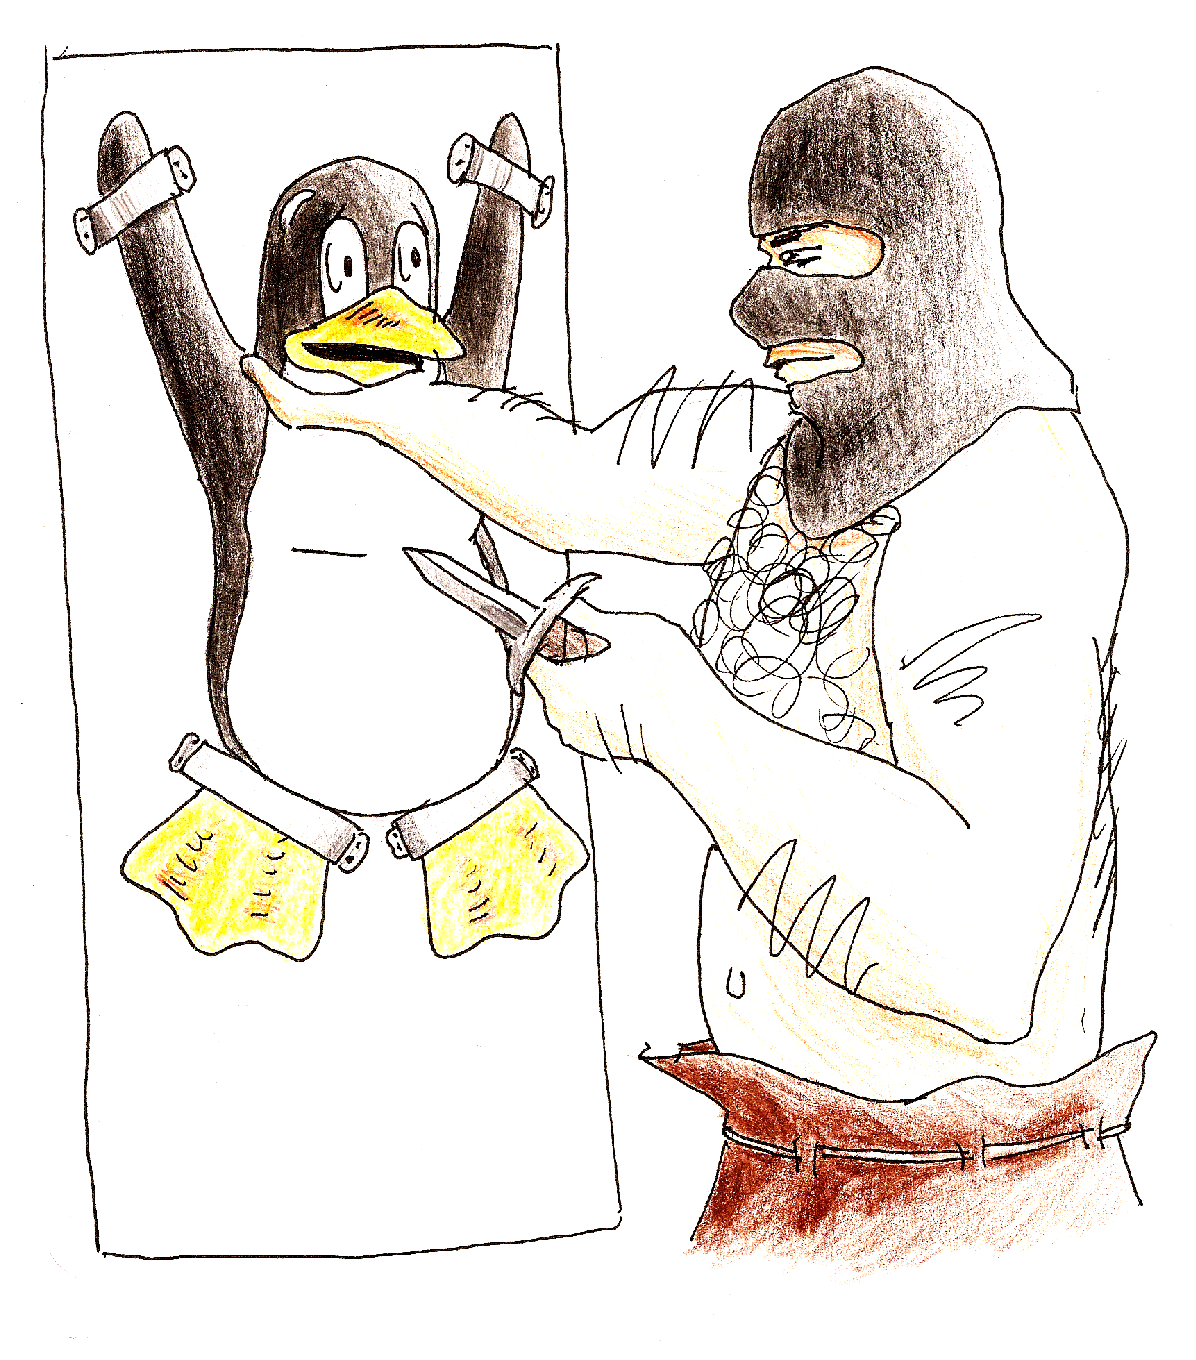
\includegraphics{cartoons/TortureTux}}
\caption{Validation and the Geneva Convention}
\ContributedBy{Figure}{fig:debugging:Validation and the Geneva Convention}{Melissa Broussard}
\end{figure}

\begin{figure}[tb]
\centering
\resizebox{2in}{!}{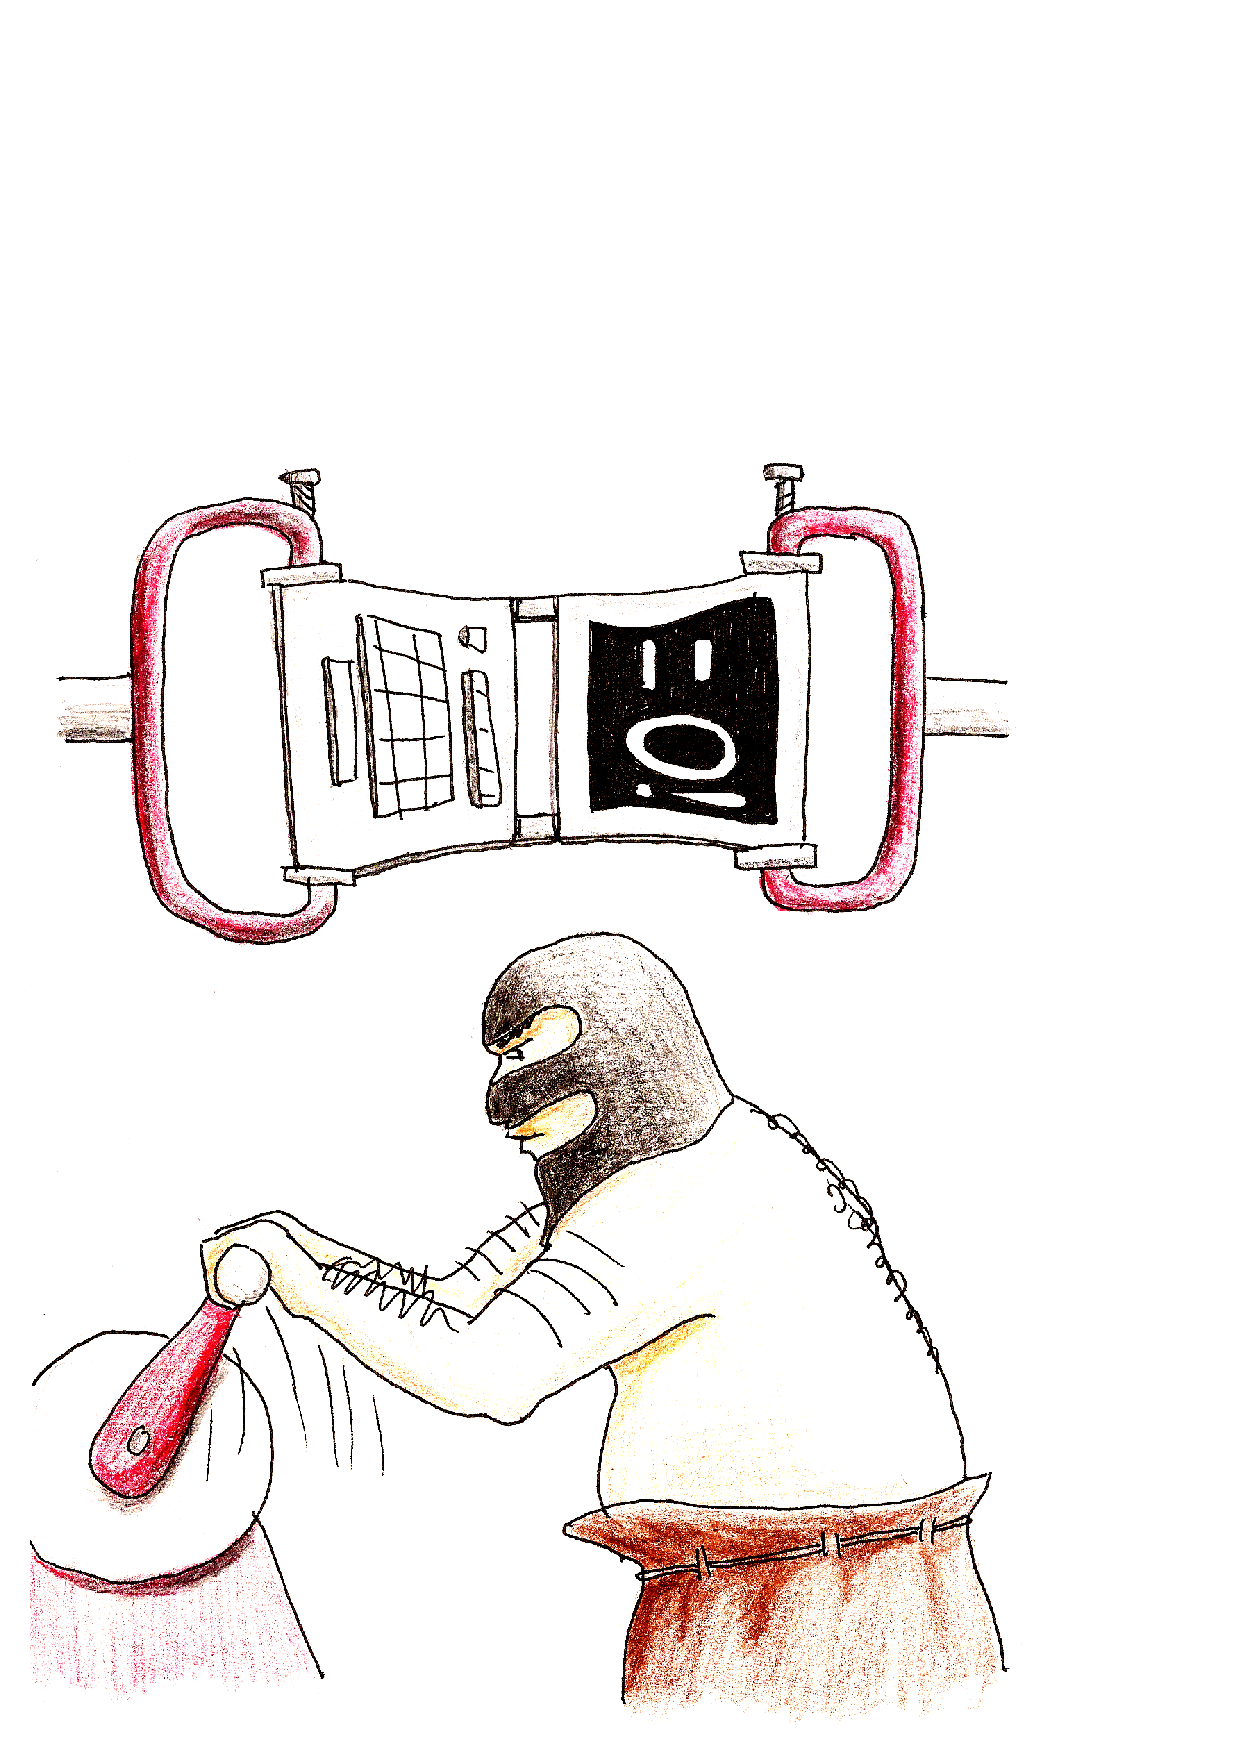
\includegraphics{cartoons/TortureLaptop}}
\caption{Rationalizing Validation}
\ContributedBy{Figure}{fig:debugging:Rationalizing Validation}{Melissa Broussard}
\end{figure}

Some people might see vigorous validation as a form of torture, as
depicted in
Figure~\ref{fig:debugging:Validation and the Geneva Convention}.\footnote{
	More cynical people might question whether these people are instead
	merely afraid that validation will find bugs that they will then
	be expected to fix.}
Such people might do well to remind themselves that, Tux cartoons aside,
they are really torturing an inanimate object, as shown in
Figure~\ref{fig:debugging:Rationalizing Validation}.
In addition, rest assured that those who fail to torture their code are
doomed to be tortured by it.

However, this leaves open the question of exactly when during the project
lifetime validation should start, a topic taken up by the next section.

\subsection{When Should Validation Start?}
\label{sec:debugging:When Should Validation Start?}

Validation should start at the same time that the project starts.

To see this, consider that tracking down a bug is much harder in a large
program than in a small one.
Therefore, to minimize the time and effort required to track down bugs,
you should test small units of code.
Although you won't find all the bugs this way, you will find a substantial
fraction, and it will be much easier to find and fix the ones you do find.
Testing at this level can also alert you to larger flaws in your overall
design, minimizing the time you waste writing code that is quite literally
broken by design.

But why wait until you have code before validating your design?\footnote{
	The old saying ``First we must code, then we have incentive to
	think'' notwithstanding.}
Hopefully reading Chapters~\ref{chp:Hardware and its Habits}
and~\ref{chp:Tools of the Trade} provided you with the information
required to avoid some regrettably common design flaws,
but discussing your design with a colleague or even simply writing it
down can help flush out additional flaws.

However, it is all too often the case that waiting to start validation
until you have a design is waiting too long.
Mightn't your natural level of optimism caused you to start the design
before you fully understood the requirements?
The answer to this question will almost always be ``yes''.
One good way to avoid flawed requirements is to get to know your users.
To really serve them well, you will have to live among them.

\QuickQuiz{}
	You are asking me to do all this validation BS before
	I even start coding???
	That sounds like a great way to never get started!!!
\QuickQuizAnswer{
	If it is your project, for example, a hobby, do what you like.
	Any time you waste will be your own, and you have no one else
	to answer to for it.
	And there is a good chance that the time will not be completely
	wasted.
	For example, if you are embarking on a first-of-a-kind project,
	the requirements are in some sense unknowable anyway.
	In this case, the best approach might be to quickly prototype
	a number of rough solutions, try them out, and see what works
	best.

	On the other hand, if you are being paid to produce a system that
	is broadly similar to existing systems, you owe it to your users,
	your employer, and your future self to validate early and often.
} \QuickQuizEnd

First-of-a-kind projects
require different approaches to validation, for example,
rapid prototyping.
Here, the main goal of the first few prototypes is to learn how
the project should be implemented, not so much to create a correct
implementation on the first try.
However, it is important to keep in mind that you should not omit
validation, but rather take a radically different approach to it.

Now that we have established that you should start validation when you
start the project, the following sections cover a number of validation
techniques and methods that have proven their worth.

\subsection{The Open Source Way}
\label{sec:debugging:The Open Source Way}

The open-source programming methodology has proven quite effective, and
includes a regimen of intense code review and testing.

I can personally attest to the effectiveness of the open-source community's
intense code review.
One of the first patches I prepared for the Linux kernel involved
a distributed filesystem where a user on one node writes to a given
file at a location that a user on another node has mapped into memory.
In this case, it is necessary to invalidate the affected pages from
the mapping in order to allow the filesystem to maintain coherence
during the write operation.
I coded up a first attempt at a patch, and, in keeping with the open-source
maxim ``post early, post often'', I posted the patch.
I then considered how I was going to test it.

But before I could even decide on an overall test strategy, I got a
reply to my posting pointing out a few bugs.
I fixed the bugs and reposted the patch, and returned to thinking
out my test strategy.
However, before I had a chance to write any test code, I received
a reply to my reposted patch, pointing out more bugs.
This process repeated itself many times, and I am not sure that I
ever got a chance to actually test the patch.

This experience brought home the truth of the open-source saying:
Given enough eyeballs, all bugs are shallow~\cite{EricSRaymond99b}.

However, when you post some code or a given patch, it is worth
asking a few questions:

\begin{enumerate}
\item	How many of those eyeballs are actually going to look at your code?
\item	How many will be experienced and clever enough to actually find
	your bugs?
\item	Exactly when are they going to look?
\end{enumerate}

I was lucky:  There was someone out there who wanted the functionality
provided by my patch, who had long experience with distributed filesystems,
and who looked at my patch almost immediately.
If no one had looked at my patch, there would have been no review, and
therefore no finding of bugs.
If the people looking at my patch had lacked experience with distributed
filesystems, it is unlikely that they would have found all the bugs.
Had they waited months or even years to look, I likely would have forgotten
how the patch was supposed to work, making it much more difficult to
fix them.

However, we must not forget the second tenet of the open-source development,
namely intensive testing.
For example, a great many people test the Linux kernel.
Some test patches as they are submitted, perhaps even yours.
Others test the -next tree, which is helpful, but there is likely to be
several weeks or even months delay between the time that you write the
patch and the time that it appears in the -next tree, by which time the
patch will not be quite as fresh in your mind.
Still others test maintainer trees, which often have a similar time delay.

Quite a few people don't test code until it is committed to mainline,
or the master source tree (Linus's tree in the case of the Linux kernel).
If your maintainer won't accept your patch until it has been tested,
this presents you with a deadlock situation: your patch won't be accepted
until it is tested, but it won't be tested until it is accepted.
Nevertheless, people who test mainline code are still relatively
aggressive, given that many people and organizations do not test code
until it has been pulled into a Linux distro.

And even if someone does test your patch, there is no guarantee that they
will be running the hardware and software configuration and workload
required to locate your bugs.

Therefore, even when writing code for an open-source project, you need to
be prepared to develop and run your own test suite.
Test development is an underappreciated and very valuable skill, so be
sure to take full advantage of any existing test suites available to
you.
Important as test development is, we will leave further discussion of it
to books dedicated to that topic.
The following sections therefore discuss locating bugs in your code given that
you already have a good test suite.

\section{Tracing}
\label{sec:debugging:Tracing}

When all else fails, add a \co{printk()}!
Or a \co{printf()}, if you are working with user-mode C-language applications.

The rationale is simple: If you cannot figure out how execution reached
a given point in the code, sprinkle print statements earlier in the
code to work out what happened.
You can get a similar effect, and with more convenience and flexibility,
by using a debugger such as gdb (for user applications) or kgdb
(for debugging Linux kernels).
Much more sophisticated tools exist, with some of the more recent
offering the ability to rewind backwards in time from the point
of failure.

These brute-force testing tools are all valuable, especially now
that typical systems have more than 64K of memory and CPUs running
faster than 4MHz.
Much has been
written about these tools, so this chapter will add little more.

However, these tools all have a serious shortcoming when the job at hand
is to convince a fastpath of a high-performance parallel algorithm
to tell you what is going wrong, namely, they often have excessive
overheads.
There are special tracing technologies for this purpose, which typically
leverage data ownership techniques
(see Chapter~\ref{chp:Data Ownership})
to minimize the overhead of runtime data collection.
One example within the Linux kernel is
``trace events''~\cite{StevenRostedt2010perfTraceEventP1,StevenRostedt2010perfTraceEventP2,StevenRostedt2010perfTraceEventP3,StevenRostedt2010perfHP+DeathlyMacros}.
Another example that handles userspace (but has not been accepted into
the Linux kernel) is LTTng~\cite{MathieuDesnoyers2009LFCollabSummit}.
Each of these uses per-CPU buffers to allow data to be collected with
extremely low overhead.
Even so, enabling tracing can sometimes change timing enough to
hide bugs, resulting in \emph{heisenbugs}, which are discussed in
Section~\ref{sec:debugging:Probability and Heisenbugs}
and especially Section~\ref{sec:debugging:Hunting Heisenbugs}.

Even if you avoid heisenbugs, other pitfalls await you.
For example, although the machine really does know all,
what it knows is almost always way more than your head can hold.
For this reason, high-quality test suites normally come with sophisticated
scripts to analyze the voluminous output.
But beware---scripts won't necessarily notice surprising things.
My rcutorture scripts are a case in point: Early versions of those
scripts were quite satisfied with a test run in which RCU grace periods
stalled indefinitely.
This of course resulted in the scripts being modified to detect RCU
grace-period stalls, but this does not change the fact that the scripts
will only detects problems that I think to make them detect.
The scripts are useful, but they are no substitute for occasional
manual scans of the rcutorture output.

Another problem with tracing and especially with \co{printk()} calls
is that their overhead is often too much for production use.
In some such cases, assertions can be helpful.

\section{Assertions}
\label{sec:debugging:Assertions}

Assertions are usually implemented in the following manner:

\vspace{5pt}
\begin{minipage}[t]{\columnwidth}
\tt
\scriptsize
\begin{verbatim}
  1 if (something_bad_is_happening())
  2   complain();
\end{verbatim}
\end{minipage}
\vspace{5pt}

This pattern is often encapsulated into C-preprocessor macros or
language intrinsics, for example, in the Linux kernel, this might
be represented as \co{WARN_ON(something_bad_is_happening())}.
Of course, if \co{something_bad_is_happening()} quite frequently,
the resulting output might obscure reports of other problems,
in which case
\co{WARN_ON_ONCE(something_bad_is_happening())} might be more appropriate.

\QuickQuiz{}
	How can you implement \co{WARN_ON_ONCE()}?
\QuickQuizAnswer{
	If you don't mind having a \co{WARN_ON_ONCE()} that
	will sometimes warn twice or three times, simply maintain
	a static variable that is initialized to zero.
	If the condition triggers, check the static variable, and
	if it is non-zero, return.
	Otherwise, set it to one, print the message, and return.

	If you really need the message to never appear more than once,
	perhaps because it is huge, you can use an atomic exchange
	operation in place of ``set it to one'' above.
	Print the message only if the atomic exchange operation returns
	zero.
} \QuickQuizEnd

In parallel code, one especially bad something that might happen is that
a function expecting to be called under a particular lock might be called
without that lock being held.
Such functions sometimes have header comments stating something like
``The caller must hold \co{foo_lock} when calling this function'', but
such a comment does no good unless someone actually reads it.
An executable statement like \co{lock_is_held(&foo_lock)} carries far
more weight.

The Linux kernel's lockdep
facility~\cite{JonathanCorbet2006lockdep,StevenRostedt2011locdepCryptic}
takes this a step farther, reporting potential deadlocks as well as
allowing functions to verify that the proper locks are held.
Of course, this additional functionality incurs significant overhead,
so that lockdep is not necessarily appropriate for production use.

So what can be done in cases where checking is necessary, but where the
overhead of runtime checking cannot be tolerated?
One approach is static analysis, which is discussed in the next section.

\section{Static Analysis}
\label{sec:debugging:Static Analysis}

Static analysis is a validation technique were one program takes a second
program as input, reporting errors and vulnerabilities located in this
second program.
Interestingly enough, almost all programs are subjected to static analysis
by their compilers or interpreters.
These tools are of course far from perfect, but their ability to locate
errors has improved immensely over the past few decades, in part because
they now have much more than 64K bytes of memory in which to carry out their
analysis.

The original UNIX \co{lint} tool~\cite{StephenJohnson1977lint} was
quite useful, though much of its functionality has since been incorporated
into C compilers.
There are nevertheless lint-like tools under development and in use to
this day.

The sparse static analyzer~\cite{JonathanCorbet2004sparse}
looks for higher-level issues in the Linux kernel, including:

\begin{enumerate}
\item	Misuse of pointers to user-space structures.
\item	Assignments from too-long constants.
\item	Empty \co{switch} statements.
\item	Mismatched lock acquisition and release primitives.
\item	Misuse of per-CPU primitives.
\item	Use of RCU primitives on non-RCU pointers and vice versa.
\end{enumerate}

Although it is likely that compilers will continue to increase their
static-analysis capabilities, the sparse static analyzer demonstrates
the benefits of static analysis outside of the compiler, particularly
for finding application-specific bugs.

\section{Code Review}
\label{sec:debugging:Code Review}

Various code-review activities are special cases of static analysis, but
with human beings doing the analysis.
This section covers inspection, walkthroughs, and self-inspection.

\subsection{Inspection}
\label{sec:debugging:Inspection}

Traditionally, formal code inspections take place in face-to-face meetings
with formally defined roles: moderator, developer, and one or two other
participants.
The developer reads through the code, explaining what it is doing and
why it works.
The one or two other participants ask questions and raise issues, while
the moderator's job is to resolve any conflicts and to take notes.
This process can be extremely effective at locating bugs, particularly
if all of the participants are familiar with the code at hand.

However, this face-to-face formal procedure does not necessarily
work well in the global Linux kernel community, although it might work
well via an IRC session.
Instead, individuals review code separately and provide comments via
email or IRC.
The note-taking is provided by email archives or IRC logs, and moderators
volunteer their services as appropriate.
Give or take the occasional flamewar, this process also works reasonably
well, particularly if all of the participants are familiar with the
code at hand.\footnote{
	That said, one advantage of the Linux kernel community approach
	over traditional formal inspections is the greater probability of
	contributions from people \emph{not} familiar with the code,
	who therefore might not be blinded by the invalid assumptions
	harbored by those familiar with the code.}

It is quite likely that the Linux kernel community's review process
is ripe for improvement:

\begin{enumerate}
\item	There is sometimes a shortage of people with the time and
	expertise required to carry out an effective review.
\item	Even though all review discussions are archived, they are
	often ``lost'' in the sense that insights are forgotten and
	people often fail to look up the discussions.
	This can result in re-insertion of the same old bugs.
\item	It is sometimes difficult to resolve flamewars when they do
	break out, especially when the combatants have disjoint
	goals, experience, and vocabulary.
\end{enumerate}

When reviewing, therefore, it is worthwhile to review relevant documentation
in commit logs, bug reports, and LWN articles.

\subsection{Walkthroughs}
\label{sec:debugging:Walkthroughs}

A traditional code walkthrough is similar to a formal inspection,
except that the group
``plays computer'' with the code, driven by specific test cases.
A typical walkthrough team has a moderator, a secretary (who records
bugs found), a testing expert (who generates the test cases) and
perhaps one to two others.
These can be extremely effective, albeit also extremely time-consuming.

It has been some decades since I have participated in a formal
walkthrough, and I suspect that a present-day walkthrough would
use single-stepping debuggers.
One could imagine a particularly sadistic procedure as follows:

\begin{enumerate}
\item	The tester presents the test case.
\item	The moderator starts the code under a debugger, using the
	specified test case as input.
\item	Before each statement is executed, the developer is required
	to predict the outcome of the statement and explain why
	this outcome is correct.
\item	If the outcome differs from that predicted by the developer,
	this is taken as evidence of a potential bug.
\item	In parallel code, a ``concurrency shark'' asks what code
	might execute concurrently with this code, and why such
	concurrency is harmless.
\end{enumerate}

Sadistic, certainly.
Effective?
Maybe.
If the participants have a good understanding of the requirements,
software tools, data structures, and algorithms, then walkthroughs
can be extremely effective.
If not, walkthroughs are often a waste of time.

\subsection{Self-Inspection}
\label{sec:debugging:Self-Inspection}

Although developers are usually not all that effective at inspecting
their own code, there are a number of situations where there is no
reasonable alternative.
For example, the developer might be the only person authorized to look
at the code, other qualified developers might all be too busy, or
the code in question might be sufficiently bizarre that the developer
is unable to convince anyone else to take it seriously until after
demonstrating a prototype.
In these cases, the following procedure can be quite helpful,
especially for complex parallel code:

\begin{enumerate}
\item	Write design document with requirements, diagrams for data structures,
	and rationale for design choices.
\item	Consult with experts, update the design document as needed.
\item	Write the code in pen on paper, correct errors as you go.
	Resist the temptation to refer to pre-existing nearly identical code
	sequences, instead, copy them.
\item	If there were errors, copy the code in pen on fresh paper, correcting
	errors as you go.
	Repeat until the last two copies are identical.
\item	Produce proofs of correctness for any non-obvious code.
\item	Where possible, test the code fragments from the bottom up.
\item	When all the code is integrated, do full-up functional and
	stress testing.
\item	Once the code passes all tests, write code-level documentation,
	perhaps as an extension to the design document discussed above.
\end{enumerate}

When I faithfully follow this procedure for new RCU code, there are
normally only a few bugs left at the end.
With a few prominent (and embarrassing)
exceptions~\cite{PaulEMcKenney2011RCU3.0trainwreck},
I usually manage to locate these bugs before others do.
That said, this is getting more difficult over time as the number and
variety of Linux-kernel users increases.

\QuickQuiz{}
	Why would anyone bother copying existing code in pen on paper???
	Doesn't that just increase the probability of transcription errors?
\QuickQuizAnswer{
	If you are worried about transcription errors, please allow me
	to be the first to introduce you to a really cool tool named
	\co{diff}.
	In addition, carrying out the copying can be quite valuable:
	\begin{enumerate}
	\item	If you are copying a lot of code, you are probably failing
		to take advantage of an opportunity for abstraction.
		The act of copying code can provide great motivation
		for abstraction.
	\item	Copying the code gives you an opportunity to think about
		whether the code really works in its new setting.
		Is there some non-obvious constraint, such as the need
		to disable interrupts or to hold some lock?
	\item	Copying the code also gives you time to consider whether
		there is some better way to get the job done.
	\end{enumerate}
	So, yes, copy the code!
} \QuickQuizEnd

\QuickQuiz{}
	This procedure is ridiculously over-engineered!
	How can you expect to get a reasonable amount of software
	written doing it this way???
\QuickQuizAnswer{
	Indeed, repeatedly copying code by hand is laborious and slow.
	However, when combined with heavy-duty stress testing and
	proofs of correctness, this approach is also extremely effective
	for complex parallel code where ultimate performance and
	reliability are required and where debugging is difficult.
	The Linux-kernel RCU implementation is a case in point.

	On the other hand, if you are writing a simple single-threaded
	shell script to manipulate some data, then you would be
	best-served by a different methodology.
	For example, you might enter each command one at a time
	into an interactive shell with a test data set to make
	sure that it did what you wanted, then copy-and-paste the
	successful commands into your script.
	Finally, test the script as a whole.

	If you have a friend or colleague who is willing to help out,
	pair programming can work very well, as can any number of
	formal design- and code-review processes.

	And if you are writing code as a hobby, then do whatever you like.

	In short, different types of software need different development
	methodologies.
} \QuickQuizEnd

The above procedure works well for new code, but what if you need to
inspect code that you have already written?
You can of course apply the above procedure for old code in the special
case where you wrote one to throw away~\cite{Brooks79},
but the following approach can also be helpful in less desperate
circumstances:

\begin{enumerate}
\item	Using your favorite documentation tool (\LaTeX{}, HTML,
	OpenOffice, or straight ASCII), describe the high-level
	design of the code in question.
	Use lots of diagrams to illustrate the data structures
	and how these structures are updated.
\item	Make a copy of the code, stripping away all comments.
\item	Document what the code does statement by statement.
\item	Fix bugs as you find them.
\end{enumerate}

This works because describing the code in detail is an excellent way to spot
bugs~\cite{GlenfordJMyers1979}.
Although this second procedure is also a good way to get your head around
someone else's code, in many cases, the first step suffices.

Although review and inspection by others is probably more efficient and
effective, the above procedures can be quite helpful in cases where
for whatever reason it is not feasible to involve others.

At this point, you might be wondering how to write parallel code without
having to do all this boring paperwork.
Here are some time-tested ways of accomplishing this:

\begin{enumerate}
\item	Write a sequential program that scales through use of
	available parallel library functions.
\item	Write sequential plug-ins for a parallel framework,
	such as map-reduce, BOINC, or a web-application server.
\item	Do such a good job of parallel design that the problem
	is fully partitioned, then just implement sequential
	program(s) that run in parallel without communication.
\item	Stick to one of the application areas (such as linear algebra)
	where tools can automatically decompose and parallelize
	the problem.
\item	Make extremely disciplined use of parallel-programming
	primitives, so that the resulting code is easily seen to be correct.
	But beware: It is always tempting to break the rules
	``just a little bit'' to gain better performance or
	scalability.
	Breaking the rules often results in general breakage.
	That is, unless you carefully do the paperwork described in this
	section.
\end{enumerate}

But the sad fact is that even if you do the paperwork or use one of
the above ways to more-or-less safely avoid paperwork,
there will be bugs.
If nothing else, more users and a greater variety of users will expose
more bugs more quickly, especially if those users are doing things
that the original developers did not consider.
The next section describes how to handle the probabilistic bugs that
occur all too commonly when validating parallel software.

\section{Probability and Heisenbugs}
\label{sec:debugging:Probability and Heisenbugs}

So your parallel program fails.
Sometimes.

But you used techniques from the earlier sections to locate
the problem and now have a fix in place!
Congratulations!!!

\begin{figure}[tb]
\centering
\resizebox{3in}{!}{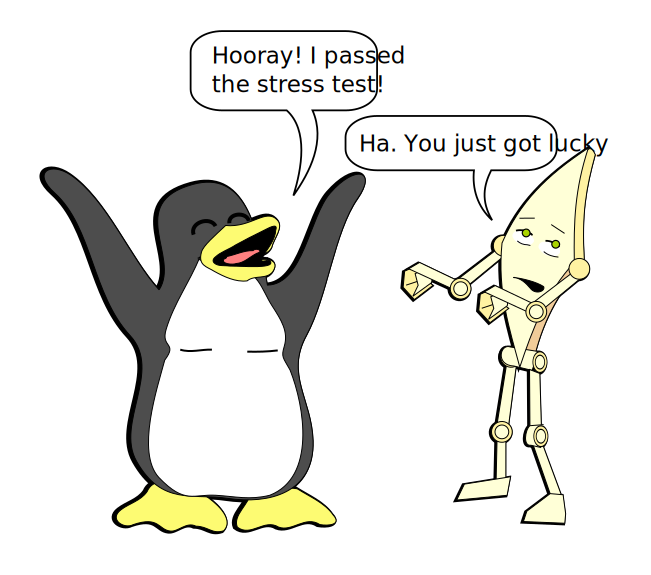
\includegraphics{cartoons/r-2014-Passed-the-stress-test}}
\caption{Passed on Merits?  Or Dumb Luck?}
\ContributedBy{Figure}{fig:cpu:Passed-the-stress-test}{Melissa Broussard}
\end{figure}

Now the question is just how much testing is required in order to be
certain that
you actually fixed the bug, as opposed to just reducing the probability
of it occurring on the one hand, having fixed only one of several
related bugs on the other hand, or made some ineffectual unrelated
change on yet a third hand.
In short, what is the answer to the eternal question posed by
Figure~\ref{fig:cpu:Passed-the-stress-test}?

Unfortunately, the honest answer is that an infinite amount of testing
is required to attain absolute certainty.

\QuickQuiz{}
	Suppose that you had a very large number of systems at your
	disposal.
	For example, at current cloud prices, you can purchase a
	huge amount of CPU time at a reasonably low cost.
	Why not use this approach to get close enough to certainty
	for all practical purposes?
\QuickQuizAnswer{
	This approach might well be a valuable addition to your
	validation arsenal.
	But it does have a few limitations:
	\begin{enumerate}
	\item	Some bugs have extremely low probabilities of occurrence,
		but nevertheless need to be fixed.
		For example, suppose that the Linux kernel's RCU
		implementation had a bug that is triggered only once
		per century of machine time on average.
		A century of CPU time is hugely expensive even on
		the cheapest cloud platforms, but we could expect
		this bug to result in more than 2,000 failures per day
		on the more than 100 million Linux instances in the
		world as of 2011.
	\item	The bug might well have zero probability of occurrence
		on your test setup, which means that you won't see it
		no matter how much machine time you burn testing it.
	\end{enumerate}
	Of course, if your code is small enough, formal validation
	may be helpful, as discussed in
	Section~\ref{chp:formal:Formal Verification}.
	But beware: formal validation of your code will not find
	errors in your assumptions, misunderstanding of the
	requirements, misunderstanding of the software or hardware
	primitives you use, or errors that you did not think to construct
	a proof for.
} \QuickQuizEnd

But suppose that we are willing to give up absolute certainty in favor
of high probability.
Then we can bring powerful statistical tools to bear on this problem.
However, this section will focus on simple statistical tools.
These tools are extremely helpful, but please note
that reading this section not a substitute
for taking a good set of statistics classes.\footnote{
	Which I most highly recommend.
	The few statistics courses I have taken have provided value
	way out of proportion to the time I spent studying for them.}

For our start with simple statistical tools, we need to decide whether
we are doing discrete or continuous testing.
Discrete testing features well-defined individual test runs.
For example, a boot-up test of a Linux kernel patch is an example
of a discrete test.
You boot the kernel, and it either comes up or it does not.
Although you might spend an hour boot-testing your kernel, the number of
times you attempted to boot the kernel and the number of times the
boot-up succeeded would often be of more interest than the length
of time you spent testing.
Functional tests tend to be discrete.

On the other hand, if my patch involved RCU, I would probably run
rcutorture, which is a kernel module that, strangely enough, tests RCU.
Unlike booting the kernel, where the appearance of a login prompt
signals the successful end of a discrete test, rcutorture will happily
continue torturing RCU until either the kernel crashes or until you
tell it to stop.
The duration of the rcutorture test is therefore (usually) of more
interest than the number of times you started and stopped it.
Therefore, rcutorture is an example of a continuous test, a category
that includes many stress tests.

The statistics governing discrete and continuous tests differ somewhat.
However, the statistics for discrete tests is simpler and more
familiar than that for continuous tests, and furthermore the
statistics for discrete tests can often be pressed into service
(with some loss of accuracy) for continuous tests.
We therefore start with discrete tests.

\subsection{Statistics for Discrete Testing}
\label{sec:debugging:Statistics for Discrete Testing}

Suppose that the bug had a 10\% chance of occurring in
a given run and that we do five runs.
How do we compute that probability of at least one run failing?
One way is as follows:

\begin{enumerate}
\item	Compute the probability of a given run succeeding, which is 90\%.
\item	Compute the probability of all five runs succeeding, which
	is 0.9 raised to the fifth power, or about 59\%.
\item	There are only two possibilities: either all five runs succeed,
	or at least one fails.
	Therefore, the probability of at least one failure is
	59\% taken away from 100\%, or 41\%.
\end{enumerate}

However, many people find it easier to work with a formula than a series
of steps, although if you prefer the above series of steps, have at it!
For those who like formulas, call the probability of a single failure $f$.
The probability of a single success is then $1-f$ and the probability
that all of $n$ tests will succeed is then:

\begin{equation}
	S_n = \left(1-f\right)^n
\end{equation}

The probability of failure is $1-S_n$, or:

\begin{equation}
	F_n = 1-\left(1-f\right)^n
\label{eq:debugging:Binomial Failure Rate}
\end{equation}

\QuickQuiz{}
	Say what???
	When I plug the earlier example of five tests each with a
	10\% failure rate into the formula, I get 59,050\% and that
	just doesn't make sense!!!
\QuickQuizAnswer{
	You are right, that makes no sense at all.

	Remember that a probability is a number between zero and one,
	so that you need to divide a percentage by 100 to get a
	probability.
	So 10\% is a probability of 0.1, which gets a probability
	of 0.4095, which rounds to 41\%, which quite sensibly
	matches the earlier result.
} \QuickQuizEnd

So suppose that a given test has been failing 10\% of the time.
How many times do you have to run the test to be 99\% sure that
your supposed fix has actually improved matters?

Another way to ask this question is ``How many times would we need
to run the test to cause the probability of failure to rise above 99\%?''
After all, if we were to run the test enough times that the probability
of seeing at least one failure becomes 99\%, if there are no failures,
there is only 1\% probability of this being due to dumb luck.
And if we plug $f=0.1$ into
Equation~\ref{eq:debugging:Binomial Failure Rate} and vary $n$,
we find that 43 runs gives us a 98.92\% chance of at least one test failing
given the original 10\% per-test failure rate,
while 44 runs gives us a 99.03\% chance of at least one test failing.
So if we run the test on our fix 44 times and see no failures, there
is a 99\% probability that our fix was actually a real improvement.

But repeatedly plugging numbers into
Equation~\ref{eq:debugging:Binomial Failure Rate}
can get tedious, so let's solve for $n$:

\begin{eqnarray}
	F_n = 1-\left(1-f\right)^n \\
	1 - F_n = \left(1-f\right)^n \\
	\log \left(1 - F_n\right) = n \; \log \left(1 - f\right)
\end{eqnarray}

Finally the number of tests required is given by:

\begin{equation}
	n = \frac{\log\left(1 - F_n\right)}{\log\left(1 - f\right)}
\label{eq:debugging:Binomial Number of Tests Required}
\end{equation}

Plugging $f=0.1$ and $F_n=0.99$ into
Equation~\ref{eq:debugging:Binomial Number of Tests Required}
gives 43.7, meaning that we need 44 consecutive successful test
runs to be 99\% certain that our fix was a real improvement.
This matches the number obtained by the previous method, which
is reassuring.

\QuickQuiz{}
	In Equation~\ref{eq:debugging:Binomial Number of Tests Required},
	are the logarithms base-10, base-2, or base-$e$?
\QuickQuizAnswer{
	It does not matter.
	You will get the same answer no matter what base of logarithms
	you use because the result is a pure ratio of logarithms.
	The only constraint is that you use the same base for both
	the numerator and the denominator.
} \QuickQuizEnd

\begin{figure}[tb]
\centering
\resizebox{2.5in}{!}{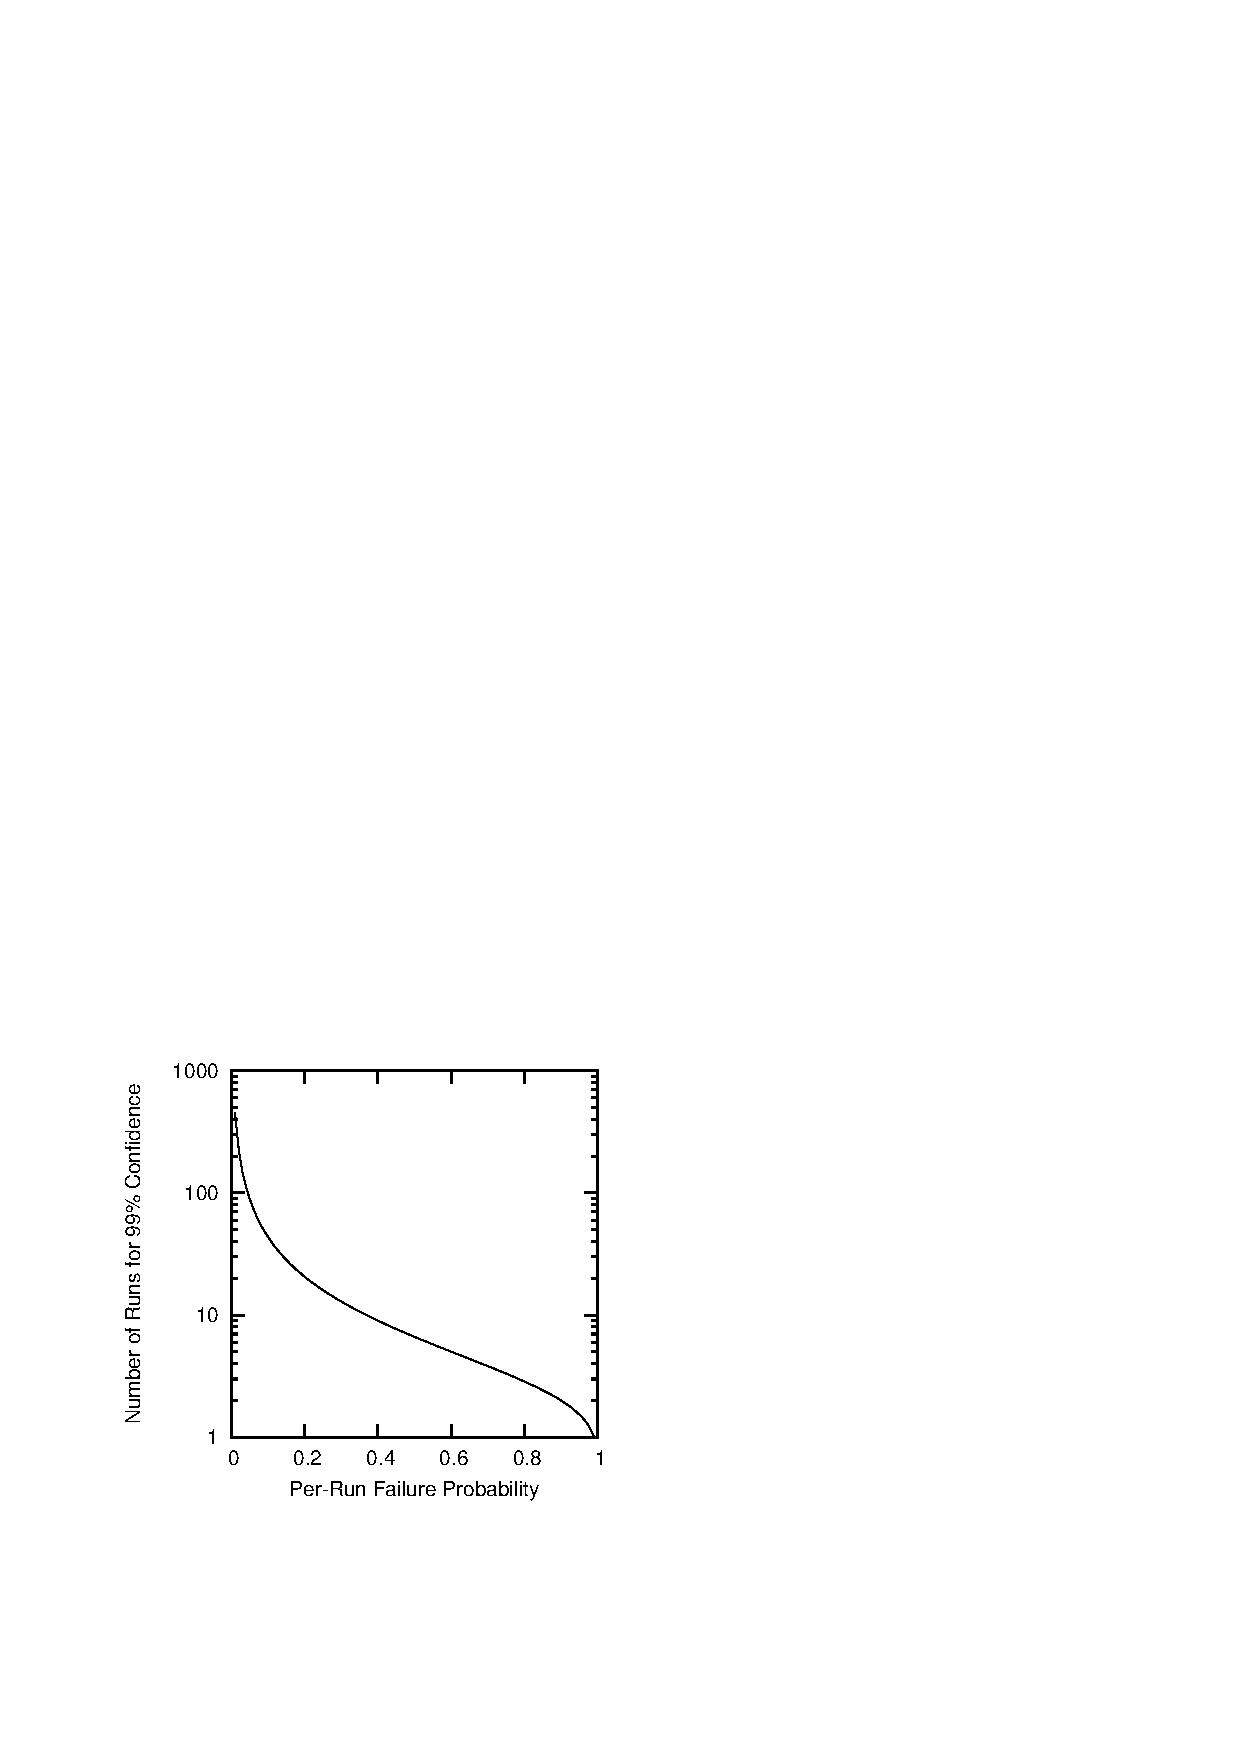
\includegraphics{CodeSamples/debugging/BinomialNRuns}}
\caption{Number of Tests Required for 99 Percent Confidence Given Failure Rate}
\label{fig:debugging:Number of Tests Required for 99 Percent Confidence Given Failure Rate}
\end{figure}

Figure~\ref{fig:debugging:Number of Tests Required for 99 Percent Confidence Given Failure Rate}
shows a plot of this function.
Not surprisingly, the less frequently each test run fails, the more
test runs are required to be 99\% confident that the bug has been
fixed.
If the bug caused the test to fail only 1\% of the time, then a
mind-boggling 458 test runs are required.
As the failure probability decreases, the number of test runs required
increases, going to infinity as the failure probability goes to zero.

The moral of this story is that when you have found a rarely occurring
bug, your testing job will be much easier if you can come up with
a carefully targeted test with a much higher failure rate.
For example, if your targeted test raised the failure rate from 1\%
to 30\%, then the number of runs required for 99\% confidence
would drop from 458 test runs to a mere thirteen test runs.

But these thirteen test runs would only give you 99\% confidence that
your fix had produced ``some improvement''.
Suppose you instead want to have 99\% confidence that your fix reduced
the failure rate by an order of magnitude.
How many failure-free test runs are required?

An order of magnitude improvement from a 30\% failure rate would be
a 3\% failure rate.
Plugging these numbers into
Equation~\ref{eq:debugging:Binomial Number of Tests Required} yields:

\begin{equation}
	n = \frac{\log\left(1 - 0.99\right)}{\log\left(1 - 0.03\right)} = 151.2
\end{equation}

So our order of magnitude improvement requires roughly an order of
magnitude more testing.
Certainty is impossible, and high probabilities are quite expensive.
Clearly making tests run more quickly and making failures more probable
are essential skills in the development of highly reliable software.
These skills will be covered in
Section~\ref{sec:debugging:Hunting Heisenbugs}.

\subsection{Abusing Statistics for Discrete Testing}
\label{sec:debugging:Abusing Statistics for Discrete Testing}

But suppose that you have a continuous test that fails about three
times every ten hours, and that you fix the bug that you believe was
causing the failure.
How long do you have to run this test without failure to be 99\% certain
that you reduced the probability of failure?

Without doing excessive violence to statistics, we could simply
redefine a one-hour run to be a discrete test that has a 30\%
probability of failure.
Then the results of in the previous section tell us that if the test
runs for 13 hours without failure, there is a 99\% probability that
our fix actually improved the program's reliability.

A dogmatic statistician might not approve of this approach, but the
sad fact is that the errors introduced by this sort of abuse of
statistical methodology are usually quite small compared to the
errors inherent in your measurements of your program's failure rates.
Nevertheless, the next section describes a slightly less dodgy approach.

\subsection{Statistics for Continuous Testing}
\label{sec:debuggingStatistics for Continuous Testing}

The fundamental formula for failure probabilities is the Poisson
distribution:

\begin{equation}
	F_m = \frac{\lambda^m}{m!} e^{-\lambda}
\label{eq:debugging:Poisson Probability}
\end{equation}

Here $F_m$ is the probability of $m$ failures in the test and
$\lambda$ is the expected failure rate per unit time.
A rigorous derivation may be found in any advanced probability
textbook, for example, Feller's classic ``An Introduction to Probability
Theory and Its Applications''~\cite{Feller58}, while a more
intuitive approach may be found in the first edition of
this book~\cite{McKenney2014ParallelProgramming-e1}.

Let's try reworking the example from
Section~\ref{sec:debugging:Abusing Statistics for Discrete Testing}
using the Poisson distribution.
Recall that this example involved a test with a 30\% failure rate per
hour, and that the question was how long the test would need to run
error-free
on a alleged fix to be 99\% certain that the fix actually reduced the
failure rate.
In this case, $\lambda$ is zero, so that
Equation~\ref{eq:debugging:Poisson Probability} reduces to:

\begin{equation}
	F_0 =  e^{-\lambda}
\end{equation}

Solving this requires setting $F_0$
to 0.01 and solving for $\lambda$, resulting in:

\begin{equation}
	\lambda = - \log 0.01 = 4.6
\end{equation}

Because we get $0.3$ failures per hour, the number of hours required
is $4.6/0.3 = 14.3$, which is within 10\% of the 13 hours
calculated using the method in
Section~\ref{sec:debugging:Abusing Statistics for Discrete Testing}.
Given that you normally won't know your failure rate to within 10\%,
this indicates that the method in
Section~\ref{sec:debugging:Abusing Statistics for Discrete Testing}
is a good and sufficient substitute for the Poisson distribution in
a great many situations.

More generally, if we have $n$ failures per unit time, and we want to
be P\% certain that a fix reduced the failure rate, we can use the
following formula:

\begin{equation}
	T = - \frac{1}{n} \log \frac{100 - P}{100}
\label{eq:debugging:Error-Free Test Duration}
\end{equation}

\QuickQuiz{}
	Suppose that a bug causes a test failure three times per hour
	on average.
	How long must the test run error-free to provide 99.9\%
	confidence that the fix significantly reduced the probability
	of failure?
\QuickQuizAnswer{
	We set $n$ to $3$ and $P$ to $99.9$ in
	Equation~\ref{eq:debugging:Error-Free Test Duration}, resulting in:

	\begin{equation}
		T = - \frac{1}{3} \log \frac{100 - 99.9}{100} = 2.3
	\end{equation}

	If the test runs without failure for 2.3 hours, we can be 99.9\%
	certain that the fix reduced the probability of failure.
} \QuickQuizEnd

As before, the less frequently the bug occurs and the greater the
required level of confidence, the longer the required error-free test run.

Suppose that a given test fails about once every hour, but after a bug
fix, a 24-hour test run fails only twice.
Assuming that the failure leading to the bug is a random occurrence,
what is the probability that the small number of
failures in the second run was due to random chance?
In other words, how confident should we be that the fix actually
had some effect on the bug?
This probability may be calculated by summing
Equation~\ref{eq:debugging:Poisson Probability} as follows:

\begin{equation}
	F_0 + F_1 + \dots + F_{m - 1} + F_m =
		\sum_{i=0}^m \frac{\lambda^i}{i!} e^{-\lambda}
\end{equation}

This is the Poisson cumulative distribution function, which can be
written more compactly as:

\begin{equation}
	F_{i \le m} = \sum_{i=0}^m \frac{\lambda^i}{i!} e^{-\lambda}
\label{eq:debugging:Possion CDF}
\end{equation}

Here $m$ is the number of errors in the long test run
(in this case, two) and $\lambda$ is expected number of errors
in the long test run (in this case, 24).
Plugging $m=2$ and $\lambda=24$ into this expression gives the probability
of two or fewer failures as about
$1.2 \times 10^{-8}$, in other words, we have a high level of confidence
that the fix actually had some relationship to the bug.\footnote{
	Of course, this result in no way excuses you from finding and
	fixing the bug(s) resulting in the remaining two failures!}

\QuickQuiz{}
	Doing the summation of all the factorials and exponentials
	is a real pain.
	Isn't there an easier way?
\QuickQuizAnswer{
	One approach is to use the open-source symbolic manipulation
	program named ``maxima''.
	Once you have installed this program, which is a part of many
	Debian-based Linux distributions, you can run it and give the
	\co{load(distrib);} command followed by any number of
	\co{bfloat(cdf_poisson(m,l));} commands, where the \co{m}
	is replaced by the desired value of $m$ and the \co{l}
	is replaced by the desired value of $\lambda$.

	In particular, the \co{bfloat(cdf_poisson(2,24));} command
	results in \co{1.181617112359357b-8}, which matches the value
	given by Equation~\ref{eq:debugging:Possion CDF}.

	Alternatively, you can use the rough-and-ready method described in
	Section~\ref{sec:debugging:Abusing Statistics for Discrete Testing}.
} \QuickQuizEnd

\QuickQuiz{}
	But wait!!!
	Given that there has to be \emph{some} number of failures
	(including the possibility of zero failures),
	shouldn't the summation shown in
	Equation~\ref{eq:debugging:Possion CDF}
	approach the value $1$ as $m$ goes to infinity?
\QuickQuizAnswer{
	Indeed it should.
	And it does.

	To see this, note that $e^{-\lambda}$ does not depend on $i$,
	which means that it can be pulled out of the summation as follows:

	\begin{equation}
		e^{-\lambda} \sum_{i=0}^\infty \frac{\lambda^i}{i!}
	\end{equation}

	The remaining summation is exactly the Taylor series for
	$e^\lambda$, yielding:

	\begin{equation}
		e^{-\lambda} e^\lambda
	\end{equation}

	The two exponentials are reciprocals, and therefore cancel,
	resulting in exactly $1$, as required.
} \QuickQuizEnd

The Poisson distribution is a powerful tool for analyzing test results,
but the fact is that in this last example there were still two remaining
test failures in a 24-hour test run.
Such a low failure rate results in very long test runs.
The next section discusses counter-intuitive ways of improving this situation.

\subsection{Hunting Heisenbugs}
\label{sec:debugging:Hunting Heisenbugs}

This line of thought also helps explain heisenbugs:
adding tracing and assertions can easily reduce the probability
of a bug appearing.
And this is why extremely lightweight tracing and assertion mechanism are
so critically important.

The name ``heisenbug'' stems from the Heisenberg Uncertainty Principle
from quantum physics, which states that it is impossible to exactly
quantify a given particle's position and velocity at any given point
in time~\cite{WeinerHeisenberg1927Uncertain}.
Any attempt to more accurately measure that particle's position will
result in increased uncertainty of its velocity.
A similar effect occurs for heisenbugs: attempts to track down the heisenbug
causes it to radically change its symptoms or even disappear completely.

If the field of physics inspired the name of this problem, it is only
logical that we should look to the field of physics for the solution.
Fortunately, particle physics is up to the task:
Why not create an anti-heisenbug to annihilate the heisenbug?

This section describes a number of ways to do just that:

\begin{enumerate}
\item	Add delay to race-prone regions.
\item	Increase workload intensity.
\item	Test suspicious subsystems in isolation.
\item	Simulate unusual events.
\item	Count near misses.
\end{enumerate}

Although producing an anti-heisenbug for a given heisenbug is more an
art than a science, the following sections give some tips on
generating the corresponding species of anti-heisenbug.

\subsubsection{Add Delay}
\label{sec:debugging:Add Delay}

Consider the count-lossy code in
Section~\ref{sec:count:Why Isn't Concurrent Counting Trivial?}.
Adding \co{printf()} statements will likely greatly reduce or even
eliminate the lost counts.
However, converting the load-add-store sequence to a load-add-delay-store
sequence will greatly increase the incidence of lost counts (try it!).
Once you spot a bug involving a race condition, it is frequently possible
to create an anti-heisenbug by adding delay in this manner.

Of course, this begs the question of how to find the race condition in
the first place.
This is a bit of a dark art, but there are a number of things you can
do to find them.

One approach is to recognize that race conditions often end up corrupting
some of the data involved in the race.
It is therefore good practice to double-check the synchronization of
any corrupted data.
Even if you cannot immediately recognize the race condition, adding
delay before and after accesses to the corrupted data might change
the failure rate.
By adding and removing the delays in an organized fashion (e.g., binary
search), you might learn more about the workings of the race condition.

\QuickQuiz{}
	How is this approach supposed to help if the corruption affected some
	unrelated pointer, which then caused the corruption???
\QuickQuizAnswer{
	Indeed, that can happen.
	Many CPUs have hardware-debugging facilities that can help you
	locate that unrelated pointer.
	Furthermore, if you have a core dump, you can search the core
	dump for pointers referencing the corrupted region of memory.
	You can also look at the data layout of the corruption, and
	check pointers whose type matches that layout.

	You can also step back and test the modules making up your
	program more intensively, which will likely confine the corruption
	to the module responsible for it.
	If this makes the corruption vanish, consider adding additional
	argument checking to the functions exported from each module.

	Nevertheless, this is a hard problem, which is why I used the
	words ``a bit of a dark art''.
} \QuickQuizEnd

Another important approach is to
vary the software and hardware configuration and look for statistically
significant differences in failure rate.
You can then look more intensively at the code implicated by the
software or hardware configuration changes that make the greatest
difference in failure rate.
It might be helpful to test that code in isolation, for example.

One important aspect of software configuration is the history of
changes, which is why \co{git bisect} is so useful.
Bisection of the change history can provide very valuable clues as
to the nature of the heisenbug.

\QuickQuiz{}
	But I did the bisection, and ended up with a huge commit.
	What do I do now?
\QuickQuizAnswer{
	A huge commit?
	Shame on you!
	This is but one reason why you are supposed to keep the commits small.

	And that is your answer: Break up the commit into bite-sized
	pieces and bisect the pieces.
	In my experience, the act of breaking up the commit is often
	sufficient to make the bug painfully obvious.
} \QuickQuizEnd

However you locate the suspicious section of code, you can then introduce
delays to attempt to increase the probability of failure.
As we have seen, increasing the probability of failure makes it much
easier to gain high confidence in the corresponding fix.

However, it is sometimes quite difficult to track down the problem using
normal debugging techniques.
The following sections present some other alternatives.

\subsubsection{Increase Workload Intensity}
\label{sec:debugging:Increase Workload Intensity}

It is often the case that a given test suite places relatively
low stress on a given subsystem, so that a small change in timing
can cause a heisenbug to disappear.
One way to create an anti-heisenbug for this case is to increase
the workload intensity, which has a good chance of increasing the
probability of the bug appearing.
If the probability is increased sufficiently, it may be possible to
add lightweight diagnostics such as tracing without causing the
bug to vanish.

How can you increase the workload intensity?
This depends on the program, but here are some things to try:

\begin{enumerate}
\item	Add more CPUs.
\item	If the program uses networking, add more network adapters
	and more or faster remote systems.
\item	If the program is doing heavy I/O when the problem occurs,
	either (1) add more storage devices, (2) use faster storage
	devices, for example, substitute SSDs for disks,
	or (3) use a RAM-based filesystem to substitute main
	memory for mass storage.
\item	Change the size of the problem, for example, if doing a parallel
	matrix multiply, change the size of the matrix.
	Larger problems may introduce more complexity, but smaller
	problems often increase the level of contention.
	If you aren't sure whether you should go large or go small,
	just try both.
\end{enumerate}

However, it is often the case that the bug is in a specific subsystem,
and the structure of the program limits the amount of stress that can
be applied to that subsystem.
The next section addresses this situation.

\subsubsection{Isolate Suspicious Subsystems}
\label{sec:debugging:Isolate Suspicious Subsystems}

If the program is structured such that it is difficult or impossible
to apply much stress to a subsystem that is under suspicion,
a useful anti-heisenbug is a stress test that tests that subsystem in
isolation.
The Linux kernel's rcutorture module takes exactly this approach with
RCU: By applying more stress to RCU than is feasible in a production
environment, the probability that any RCU bugs will be found during
rcutorture testing rather than during production use is increased.\footnote{
	Though sadly not increased to probability one.}

In fact, when creating a parallel program, it is wise to stress-test
the components separately.
Creating such component-level stress tests can seem like a waste of time,
but a little bit of component-level testing can save a huge amount
of system-level debugging.

\subsubsection{Simulate Unusual Events}
\label{sec:debugging:Simulate Unusual Events}

Heisenbugs are sometimes due to unusual events, such as
memory-allocation failure, conditional-lock-acquisition failure,
CPU-hotplug operations, timeouts, packet losses, and so on.
One way to construct an anti-heisenbug for this class of heisenbug
is to introduce spurious failures.

For example, instead of invoking \co{malloc()} directly, invoke
a wrapper function that uses a random number to decide whether
to return \co{NULL} unconditionally on the one hand, or to actually
invoke \co{malloc()} and return the resulting pointer on the other.
Inducing spurious failures is an excellent way to bake robustness into
sequential programs as well as parallel programs.

\QuickQuiz{}
	Why don't existing conditional-locking primitives provide this
	spurious-failure functionality?
\QuickQuizAnswer{
	There are locking algorithms that depend on conditional-locking
	primitives telling them the truth.
	For example, if conditional-lock failure signals that
	some other thread is already working on a given job,
	spurious failure might cause that job to never get done,
	possibly resulting in a hang.
} \QuickQuizEnd

\subsubsection{Count Near Misses}
\label{sec:debugging:Count Near Misses}

Bugs are often an all-or-nothing thing, so that either the bug happens
or it doesn't, with nothing in between.
However, it is sometimes possible to define a \emph{near miss} where
the bug does not result in a failure, but has likely manifested.
For example, suppose your code is making a robot walk.
The robot's falling over constitutes a bug in your program, but
stumbling and recovering might constitute a near miss.
If the robot falls over only once per hour, but stumbles every few
minutes, you might be able to speed up your debugging progress by
counting the number of stumbles in addition to the number of falls.

In concurrent programs, timestamping can sometimes be used to detect
near misses.
For example, locking primitives incur significant delays, so if there is
a too-short delay between a pair of operations that are supposed
to be protected by different acquisitions of the same lock, this too-short
delay might be counted as a near miss.\footnote{
	Of course, in this case, you might be better off using
	whatever \co{lock_held()} primitive is available
	in your environment.
	If there isn't a \co{lock_held()} primitive, create one!}

\begin{figure}[tbp]
\centering
\resizebox{3in}{!}{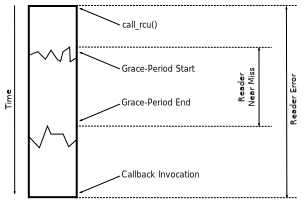
\includegraphics{debugging/RCUnearMiss}}
\caption{RCU Errors and Near Misses}
\label{fig:debugging:RCU Errors and Near Misses}
\end{figure}

For example, a low-probability bug in RCU priority boosting occurred
roughly once every hundred hours of focused rcutorture testing.
Because it would take almost 500 hours of failure-free testing to be
99\% certain that the bug's probability had been significantly reduced,
the \co{git bisect} process
to find the failure would be painfully slow---or would require an extremely
large test farm.
Fortunately, the RCU operation being tested included not only a wait for
an RCU grace period, but also a previous wait for the grace period to start
and a subsequent wait for an RCU callback to be
invoked after completion of the RCU grace period.
This distinction between an \co{rcutorture} error and near miss is
shown in
Figure~\ref{fig:debugging:RCU Errors and Near Misses}.
To qualify as a full-fledged error, an RCU read-side critical section
must extend from the \co{call_rcu()} that initiated a grace period,
through the remainder of the previous grace period, through the
entirety of the grace period initiated by the \co{call_rcu()}
(denoted by the region between the jagged lines), and
through the delay from the end of that grace period to the callback
invocation, as indicated by the ``Error'' arrow.
However, the formal definition of RCU prohibits RCU read-side critical
sections from extending across a single grace period, as indicated by
the ``Near Miss'' arrow.
This suggests using near misses as the error condition, however, this
can be problematic because different CPUs can have different opinions
as to exactly where a given
grace period starts and ends, as indicated by the jagged lines.\footnote{
	The jaggedness of these lines is seriously understated because
	idle CPUs might well be completely unaware of the most recent
	few hundred grace periods.}
Using the near misses as the error condition could therefore result
in false positives, which need to be avoided in the automated
\co{rcutorture} testing.

By sheer dumb luck, \co{rcutorture} happens to include some statistics that
are sensitive to the near-miss version of the grace period.
As noted above, these statistics are subject to false positives due to
their unsynchronized access to RCU's state variables,
but these false positives turn out to be extremely rare on strongly
ordered systems such as the IBM mainframe and x86, occurring less than
once per thousand hours of testing.

These near misses occurred roughly once per hour, about two orders of
magnitude more frequently than the actual errors.
Use of these near misses allowed the bug's root cause to be identified
in less than a week and a high degree of confidence in the fix to be
built in less than a day.
In contrast, excluding the near misses in favor of the real errors would
have required months of debug and validation time.

To sum up near-miss counting, the general approach is to replace counting
of infrequent failures with more-frequent near misses that are believed
to be correlated with those failures.
These near-misses can be considered an anti-heisenbug to the real failure's
heisenbug because the near-misses, being more frequent, are likely to
be more robust in the face of changes to your code, for example, the
changes you make to add debugging code.

Thus far, we have focused solely on bugs in the parallel program's
functionality.
However, because performance is a first-class requirement for a
parallel program (otherwise, why not write a sequential program?),
the next section looks into finding performance bugs.

\section{Performance Estimation}
\label{sec:debugging:Performance Estimation}

Parallel programs usually have performance and scalability requirements,
after all, if performance is not an issue, why not use a sequential
program?
Ultimate performance and linear scalability might not be necessary, but
there is little use for a parallel program that runs slower than its
optimal sequential counterpart.
And there really are cases where every microsecond matters and every
nanosecond is needed.
Therefore, for parallel programs, insufficient performance is just as
much a bug as is incorrectness.

\QuickQuiz{}
	That is ridiculous!!!
	After all, isn't getting the correct answer later than one would like
	better than getting an incorrect answer???
\QuickQuizAnswer{
	This question fails to consider the option of choosing not to
	compute the answer at all, and in doing so, also fails to consider
	the costs of computing the answer.
	For example, consider short-term weather forecasting, for which
	accurate models exist, but which require large (and expensive)
	clustered supercomputers, at least if you want to actually run
	the model faster than the weather.

	And in this case, any performance bug that prevents the model from
	running faster than the actual weather prevents any forecasting.
	Given that the whole purpose of purchasing the large clustered
	supercomputers was to forecast weather, if you cannot run the
	model faster than the weather, you would be better off not running
	the model at all.

	More severe examples may be found in the area of safety-critical
	real-time computing.
} \QuickQuizEnd

\QuickQuiz{}
	But if you are going to put in all the hard work of parallelizing
	an application, why not do it right?
	Why settle for anything less than optimal performance and
	linear scalability?
\QuickQuizAnswer{
	Although I do heartily salute your spirit and aspirations,
	you are forgetting that there may be high costs due to delays
	in the program's completion.
	For an extreme example, suppose that a 40\% performance shortfall
	from a single-threaded application is causing one person to die
	each day.
	Suppose further that in a day you could hack together a
	quick and dirty
	parallel program that ran 50\% faster on an eight-CPU system
	than the sequential version, but that an optimal parallel
	program would require four months of painstaking design, coding,
	debugging, and tuning.

	It is safe to say that more than 100 people would prefer the
	quick and dirty version.
} \QuickQuizEnd

Validating a parallel program must therfore include validating its
performance.
But validating performance means having a workload to run and performance
criteria with which to evaluate the program at hand.
These needs are often met by \emph{performance benchmarks}, which
are discussed in the next section.

\subsection{Benchmarking}
\label{sec:debugging:Benchmarking}

The old saying goes ``There are lies, damn lies, statistics,
and benchmarks.''
However, benchmarks are heavily used, so it is not helpful to
be too dismissive of them.

Benchmarks span the range from ad hoc test jigs to international
standards, but regardless of their level of formality, benchmarks
serve four major purposes:

\begin{enumerate}
\item	Providing a fair framework for comparing competing implementations.
\item	Focusing competitive energy on improving implementations in ways
	that matter to users.
\item	Serving as example uses of the implementations being benchmarked.
\item	Serving as a marketing tool to highlight your software's
	strong points against your competitors' offerings.
\end{enumerate}

Of course,  the only completely fair framework is the intended
application itself.
So why would anyone who cared about fairness in benchmarking
bother creating imperfect benchmarks rather than simply
using the application itself as the benchmark?

Running the actual application is in fact the best approach where it is practical.
Unfortunately, it is often impractical for the following reasons:

\begin{enumerate}
\item	The application might be proprietary, and you
	might not have the right to run the intended application.
\item	The application might require more hardware
	that you have no access to.
\item	The application might use data that you cannot legally
	access, for example, due to privacy regulations.
\end{enumerate}

In these cases, creating a benchmark that approximates
the application can help overcome these obstacles.
A carefully constructed benchmark can help promote performance,
scalability, energy efficiency, and much else besides.

\subsection{Profiling}
\label{sec:debugging:Profiling}

In many cases, a fairly small portion of your software is responsible
for the majority of the performance and scalability shortfall.
However, developers are notoriously unable to identify the actual
bottlenecks by hand.
For example, in the case of a kernel buffer allocator, all attention focused
on a search of a dense array which turned out to represent only
a few percent of the allocator's execution time.
An execution profile collected via a logic analyzer focused attention
on the cache misses that were actually responsible for the majority
of the problem~\cite{McKenney93}.

An old-school but quite effective method of tracking down performance
and scalability bugs is to run your programmer under a debugger,
then periodically interrupt it, recording the stacks of all threads
at each interruption.
The theory here is that if something is slowing down your program,
it has to be visible in your threads' executions.

That said, there are a number of tools
that will usually do a much better job of helping you to focus your
attention where it will do the most good.
Two popular choices are \co{gprof} and \co{perf}.
To use \co{perf} on a single-process program, prefix your command
with \co{perf record}, then after the command completes, type
\co{perf report}.
There is a lot of work on tools for performance debugging of multi-threaded
programs, which should make this important job easier.

\subsection{Differential Profiling}
\label{sec:debugging:Differential Profiling}

Scalability problems will not necessarily be apparent unless you are running
on very large systems.
However, it is sometimes possible to detect impending scalability problems
even when running on much smaller systems.
One technique for doing this is called \emph{differential profiling}.

The idea is to run your workload under two different sets of conditions.
For example, you might run it on two CPUs, then run it again on four
CPUs.
You might instead vary the load placed on the system, the number of
network adapters, the number of mass-storage devices, and so on.
You then collect profiles of the two runs, and mathematically combine
corresponding profile measurements.
For example, if your main concern is scalability, you might take the
ratio of corresponding measurements, and then sort the ratios into
descending numerical order.
The prime scalability suspects will then be sorted to the top of the
list~\cite{McKenney95a,McKenney99b}.

Some tools such as \co{perf} have built-in differential-profiling
support.

\subsection{Microbenchmarking}
\label{sec:debugging:Microbenchmarking}

Microbenchmarking can be useful when deciding which algorithms or
data structures are worth incorporating into a larger body of software
for deeper evaluation.

One common approach to microbenchmarking is to measure the time,
run some number of iterations of the code
under test, then measure the time again.
The difference between the two times divided by the number of iterations
gives the measured time required to execute the code under test.

Unfortunately, this approach to measurement allows any number of errors
to creep in, including:

\begin{enumerate}
\item	The measurement will include some of the overhead of
	the time measurement.
	This source of error can be reduced to an arbitrarily small
	value by increasing the number of iterations.
\item	The first few iterations of the test might incur cache misses
	or (worse yet) page faults that might inflate the measured
	value.
	This source of error can also be reduced by increasing the
	number of iterations, or it can often be eliminated entirely
	by running a few warm-up iterations before starting the
	measurement period.
\item	Some types of interference, for example, random memory errors,
	are so rare that they can be dealt with by running a number
	of sets of iterations of the test.
	If the level of interference was statistically significant,
	any performance outliers could be rejected statistically.
\item	Any iteration of the test might be interfered with by other
	activity on the system.
	Sources of interference include other applications, system
	utilities and daemons, device interrupts, firmware interrupts
	(including system management interrupts, or SMIs),
	virtualization, memory errors, and much else besides.
	Assuming that these sources of interference occur randomly,
	their effect can be minimized by reducing the number of
	iterations.
\end{enumerate}

The first and fourth sources of interference provide conflicting advice,
which is one sign that we are living in the real world.
The remainder of this section looks at ways of resolving this conflict.

\QuickQuiz{}
	But what about other sources of error, for example, due to
	interactions between caches and memory layout?
\QuickQuizAnswer{
	Changes in memory layout can indeed result in unrealistic
	decreases in execution time.
	For example, suppose that a given microbenchmark almost
	always overflows the L0 cache's associativity, but with just the right
	memory layout, it all fits.
	If this is a real concern, consider running your microbenchmark
	using huge pages (or within the kernel or on bare metal) in
	order to completely control the memory layout.
} \QuickQuizEnd

The following sections discuss ways of dealing with these measurement
errors, with
Section~\ref{sec:debugging:Isolation}
covering isolation techniques that may be used to prevent some forms of
interference,
and with
Section~\ref{sec:debugging:Detecting Interference}
covering methods for detecting interference so as to reject measurement
data that might have been corrupted by that interference.

\subsection{Isolation}
\label{sec:debugging:Isolation}

The Linux kernel provides a number of ways to isolate a group of
CPUs from outside interference.

First, let's look at interference by other processes, threads, and tasks.
The POSIX \co{sched_setaffinity()} system call may be used to move
most tasks off of a given set of CPUs and to confine your tests to
that same group.
The Linux-specific user-level \co{taskset} command may be used for
the same purpose, though both \co{sched_setaffinity()} and
\co{taskset} require elevated permissions.
Linux-specific control groups (cgroups) may be used for this same purpose.
This approach can be quite effective at reducing interference, and
is sufficient in many cases.
However, it does have limitations, for example, it cannot do anything
about the per-CPU kernel threads that are often used for housekeeping
tasks.

One way to avoid interference from per-CPU kernel threads is to run
your test at a high real-time priority, for example, by using
the POSIX \co{sched_setscheduler()} system call.
However, note that if you do this, you are implicitly taking on
responsibility for avoiding infinite loops, because otherwise
your test will prevent part of the kernel from functioning.\footnote{
	This is an example of the Spiderman Principle: ``With great
	power comes great responsibility.''}

These approaches can greatly reduce, and perhaps even eliminate,
interference from processes, threads, and tasks.
However, it does nothing to prevent interference from device
interrupts, at least in the absence of threaded interrupts.
Linux allows some control of threaded interrupts via the
\path{/proc/irq} directory, which contains numerical directories, one
per interrupt vector.
Each numerical directory contains \co{smp_affinity} and
\co{smp_affinity_list}.
Given sufficient permissions, you can write a value to these files
to restrict interrupts to the specified set of CPUs.
For example, ``\co{sudo echo 3 > /proc/irq/23/smp_affinity}''
would confine interrupts on vector~23 to CPUs~0 and~1.
The same results may be obtained via
``\co{sudo echo 0-1 > /proc/irq/23/smp_affinity_list}''.
You can use ``\co{cat /proc/interrupts}'' to obtain a list of the interrupt
vectors on your system, how many are handled by each CPU, and what
devices use each interrupt vector.

Running a similar command for all interrupt vectors on your system
would confine interrupts to CPUs~0 and~1, leaving the remaining CPUs
free of interference.
Or mostly free of interference, anyway.
It turns out that the scheduling-clock interrupt fires on each CPU
that is running in user mode.\footnote{
	Frederic Weisbecker is working on an adaptive-ticks project
	that will allow the scheduling-clock interrupt to be shut
	off on any CPU that has only one runnable task, but as of
	early 2013, this is unfortunately still work in progress.}
In addition you must take care to ensure that the set of CPUs that you
confine the interrupts to is capable of handling the load.

But this only handles processes and interrupts running in the same
operating-system instance as the test.
Suppose that you are running the test in a guest OS that is itself
running on a hypervisor, for example, Linux running KVM?
Although you can in theory apply the same techniques at the hypervisor
level that you can at the guest-OS level, it is quite common for
hypervisor-level operations to be restricted to authorized personnel.
In addition, none of these techniques work against firmware-level
interference.

\QuickQuiz{}
	Wouldn't the techniques suggested to isolate the code under
	test also affect that code's performance, particularly if
	it is running within a larger application?
\QuickQuizAnswer{
	Indeed it might, although in most microbenchmarking efforts
	you would extract the code under test from the enclosing
	application.
	Nevertheless, if for some reason you must keep the code under
	test within the application, you will very likely need to use
	the techniques discussed in
	Section~\ref{sec:debugging:Detecting Interference}.
} \QuickQuizEnd

If you find yourself in this painful situation, instead of preventing
the interference, you might need to detect the interference as described
in the next section.

\subsection{Detecting Interference}
\label{sec:debugging:Detecting Interference}

If you cannot prevent interference, perhaps you can detect the
interference after the fact and reject the test runs that were affected
by that interference.
Section~\ref{sec:debugging:Detecting Interference Via Measurement}
describes methods of rejection involving additional measurements,
while Section~\ref{sec:debugging:Detecting Interference Via Statistics}
describes statistics-based rejection.

\subsubsection{Detecting Interference Via Measurement}
\label{sec:debugging:Detecting Interference Via Measurement}

%	Sources of interference include other applications, system
%	utilities and daemons, device interrupts, firmware interrupts
%	(including system management interrupts, or SMIs),
%	virtualization, memory errors, and much else besides.

Many systems, including Linux, provide means for determining after the
fact whether some forms of interference have occurred.
For example, if your test encountered process-based interference,
a context switch must have occurred during the test.
On Linux-based systems, this context switch will be visible in
\path{/proc/<PID>/sched} in the \co{nr_switches} field.
Similarly, interrupt-based interference can be detected via the
\path{/proc/interrupts} file.

{ \scriptsize
\begin{verbbox}
  1 #include <sys/time.h>
  2 #include <sys/resource.h>
  3 
  4 /* Return 0 if test results should be rejected. */
  5 int runtest(void)
  6 {
  7   struct rusage ru1;
  8   struct rusage ru2;
  9 
 10   if (getrusage(RUSAGE_SELF, &ru1) != 0) {
 11     perror("getrusage");
 12     abort();
 13   }
 14   /* run test here. */
 15   if (getrusage(RUSAGE_SELF, &ru2 != 0) {
 16     perror("getrusage");
 17     abort();
 18   }
 19   return (ru1.ru_nvcsw == ru2.ru_nvcsw &&
 20     ru1.runivcsw == ru2.runivcsw);
 21 }
\end{verbbox}
}
\begin{figure}[tb]
\centering
\theverbbox
\caption{Using getrusage() to Detect Context Switches}
\label{fig:count:Using getrusage() to Detect Context Switches}
\end{figure}

Opening and reading files is not the way to low overhead, and it is
possible to get the count of context switches for a given thread
by using the \co{getrusage()} system call, as shown in
Figure~\ref{fig:count:Using getrusage() to Detect Context Switches}.
This same system call can be used to detect minor page faults (\co{ru_minflt})
and major page faults (\co{ru_majflt}).

Unfortunately, detecting memory errors and firmware interference is quite
system-specific, as is the detection of interference due to virtualization.
Although avoidance is better than detection, and detection is better than
statistics, there are times when one must avail oneself of statistics,
a topic addressed in the next section.

\subsubsection{Detecting Interference Via Statistics}
\label{sec:debugging:Detecting Interference Via Statistics}

Any statistical analysis will be based on assumptions about the data,
and performance microbenchmarks often support the following assumptions:

\begin{enumerate}
\item	Smaller measurements are more likely to be accurate than
	larger measurements.
\item	The measurement uncertainty of good data is known.
\item	A reasonable fraction of the test runs will result in good data.
\end{enumerate}

The fact that smaller measurements are more likely to be accurate than
larger measurements suggests that sorting the measurements in increasing
order is likely to be productive.\footnote{
	To paraphrase the old saying, ``Sort first and ask questions later.''}
The fact that the measurement uncertainty is known allows us to accept
measurements within this uncertainty of each other:  If the effects of
interference are large compared to this uncertainty, this will ease
rejection of bad data.
Finally, the fact that some fraction (for example, one third) can be
assumed to be good allows us to blindly accept the first portion of the
sorted list, and this data can then be used to gain an estimate of the
natural variation of the measured data, over and above the assumed
measurement error.

The approach is to take the specified number of leading elements from the
beginning of the sorted list, and use these to estimate a typical
inter-element delta, which in turn may be multiplied by the number of
elements in the list to obtain an upper bound on permissible values.
The algorithm then repeatedly considers the next element of the list.
If it falls below the upper bound, and if the distance between
the next element and the previous element is not too much greater than
the average inter-element distance for the portion of the list accepted
thus far, then the next element is accepted and the process repeats.
Otherwise, the remainder of the list is rejected.

{ \scriptsize
\begin{verbbox}
  1 divisor=3
  2 relerr=0.01
  3 trendbreak=10
  4 while test $# -gt 0
  5 do
  6   case "$1" in
  7   --divisor)
  8     shift
  9     divisor=$1
 10     ;;
 11   --relerr)
 12     shift
 13     relerr=$1
 14     ;;
 15   --trendbreak)
 16     shift
 17     trendbreak=$1
 18     ;;
 19   esac
 20   shift
 21 done
 22 
 23 awk -v divisor=$divisor -v relerr=$relerr \
 24     -v trendbreak=$trendbreak '{
 25   for (i = 2; i <= NF; i++)
 26     d[i - 1] = $i;
 27   asort(d);
 28   i = int((NF + divisor - 1) / divisor);
 29   delta = d[i] - d[1];
 30   maxdelta = delta * divisor;
 31   maxdelta1 = delta + d[i] * relerr;
 32   if (maxdelta1 > maxdelta)
 33     maxdelta = maxdelta1;
 34   for (j = i + 1; j < NF; j++) {
 35     if (j <= 2)
 36       maxdiff = d[NF - 1] - d[1];
 37     else
 38       maxdiff = trendbreak * \
 39       (d[j - 1] - d[1]) / (j - 2);
 40     if (d[j] - d[1] > maxdelta && \
 41         d[j] - d[j - 1] > maxdiff)
 42       break;
 43   }
 44   n = sum = 0;
 45   for (k = 1; k < j; k++) {
 46     sum += d[k];
 47     n++;
 48   }
 49   min = d[1];
 50   max = d[j - 1];
 51   avg = sum / n;
 52   print $1, avg, min, max, n, NF - 1;
 53 }'
\end{verbbox}
}
\begin{figure}[tb]
\centering
\theverbbox
\caption{Statistical Elimination of Interference}
\label{fig:count:Statistical Elimination of Interference}
\end{figure}

Figure~\ref{fig:count:Statistical Elimination of Interference}
shows a simple \co{sh}/\co{awk} script implementing this notion.
Input consists of an x-value followed by an arbitrarily long list of y-values,
and output consists of one line for each input line, with fields as follows:

\begin{enumerate}
\item	The x-value.
\item	The average of the selected data.
\item	The minimum of the selected data.
\item	The maximum of the selected data.
\item	The number of selected data items.
\item	The number of input data items.
\end{enumerate}

This script takes three optional arguments as follows:

\begin{itemize}
\item	\co{--divisor}: Number of segments to divide the list into,
	for example, a divisor of four means that the first quarter
	of the data elements will be assumed to be good.
	This defaults to three.
\item	\co{--relerr}: Relative measurement error.  The script assumes
	that values that differ by less than this error are for all
	intents and purposes equal.
	This defaults to 0.01, which is equivalent to 1\%.
\item	\co{--trendbreak}: Ratio of inter-element spacing constituting
	a break in the trend of the data.
	For example, if the average spacing in the data accepted so far
	is 1.5, then if the trend-break ratio is 2.0, then if the next
	data value differs from the last one by more than 3.0, this
	constitutes a break in the trend.
	(Unless of course, the relative error is greater than 3.0, in
	which case the ``break'' will be ignored.)
\end{itemize}

Lines~1-3 of
Figure~\ref{fig:count:Statistical Elimination of Interference}
set the default values for the parameters, and lines~4-21 parse
any command-line overriding of these parameters.
The \co{awk} invocation on lines~23 and~24 sets the values of the
\co{divisor}, \co{relerr}, and \co{trendbreak} variables to their
\co{sh} counterparts.
In the usual \co{awk} manner, lines~25-52 are executed on each input
line.
The loop spanning lines~24 and~26 copies the input y-values to the
\co{d} array, which line~27 sorts into increasing order.
Line~28 computes the number of y-values that are to be trusted absolutely
by applying \co{divisor} and rounding up.

Lines~29-33 compute the \co{maxdelta} value used as a lower bound on
the upper bound of y-values.
To this end, lines~29 and~30 multiply the difference in values over
the trusted region of data by the \co{divisor}, which projects the
difference in values across the trusted region across the entire
set of y-values.
However, this value might well be much smaller than the relative error,
so line~31 computes the absolute error (\co{d[i] * relerr}) and adds
that to the difference \co{delta} across the trusted portion of the data.
Lines~32 and~33 then compute the maximum of these two values.

Each pass through the loop spanning lines~34-43 attempts to add another
data value to the set of good data.
Lines 35-39 compute the trend-break delta, with line~36 disabling this
limit if we don't yet have enough values to compute a trend,
and with lines~38 and~39 multiplying \co{trendbreak} by the average
difference between pairs of data values in the good set.
If line~40 determines that the candidate data value would exceed the
lower bound on the upper bound (\co{maxdelta}) \emph{and}
line~41 determines that the difference between the candidate data value
and its predecessor exceeds the trend-break difference (\co{maxdiff}),
then line~42 exits the loop: We have the full good set of data.

Lines~44-52 then compute and print the statistics for the data set.

\QuickQuiz{}
	This approach is just plain weird!
	Why not use means and standard deviations, like we were taught
	in our statistics classes?
\QuickQuizAnswer{
	Because mean and standard deviation were not designed to do this job.
	To see this, try applying mean and standard deviation to the
	following data set, given a 1\% relative error in measurement:

	\begin{quote}
		49,548.4 49,549.4 49,550.2 49,550.9 49,550.9 49,551.0
		49,551.5 49,552.1 49,899.0 49,899.3 49,899.7 49,899.8
		49,900.1 49,900.4 52,244.9 53,333.3 53,333.3 53,706.3
		53,706.3 54,084.5
	\end{quote}

	The problem is that mean and standard deviation do not rest on
	any sort of measurement-error assumption, and they will therefore
	see the difference between the values near 49,500 and those near
	49,900 as being statistically significant, when in fact they are
	well within the bounds of estimated measurement error.

	Of course, it is possible to create a script similar to
	that in
	Figure~\ref{fig:count:Statistical Elimination of Interference}
	that uses standard deviation rather than absolute difference
	to get a similar effect,
	and this is left as an exercise for the interested reader.
	Be careful to avoid divide-by-zero errors arising from strings
	of identical data values!
} \QuickQuizEnd

\QuickQuiz{}
	But what if all the y-values in the trusted group of data
	are exactly zero?
	Won't that cause the script to reject any non-zero value?
\QuickQuizAnswer{
	Indeed it will!
	But if your performance measurements often produce a value of
	exactly zero, perhaps you need to take a closer look at your
	performance-measurement code.

	Note that many approaches based on mean and standard deviation
	will have similar problems with this sort of dataset.
} \QuickQuizEnd

Although statistical interference detection can be quite useful, it should
be used only as a last resort.
It is far better to avoid interference in the first place
(Section~\ref{sec:debugging:Isolation}), or, failing that,
detecting interference via measurement
(Section~\ref{sec:debugging:Detecting Interference Via Measurement}).

\section{Summary}
\label{sec:debugging:Summary}

\begin{figure}[tbhp]
\centering
\resizebox{3in}{!}{\includegraphics{cartoons/UseTheRightCannon}}
\caption{Choose Validation Methods Wisely}
\ContributedBy{Figure}{fig:debugging:Choose Validation Methods Wisely}{Melissa Broussard}
\end{figure}

Although validation never will be an exact science, much can be gained
by taking an organized approach to it, as an organized approach will
help you choose the right validation tools for your job, avoiding
situations like the one fancifully depicted in
Figure~\ref{fig:debugging:Choose Validation Methods Wisely}.

A key choice is that of statistics.
Although the methods described in this chapter work very well most of
the time, they do have their limitations.
These limitations are inherent because we are attempting to do something
that is in general impossible, courtesy of the
Halting Problem~\cite{AlanMTuring1937HaltingProblem,GeoffreyKPullum2000HaltingProblem}.
Fortunately for us, there are a huge number of special cases in which
we can not only work out whether a given program will halt, but also
establish estimates for how long it will run before halting, as discussed in
Section~\ref{sec:debugging:Performance Estimation}.
Furthermore, in cases where a given program might or might not work
correctly, we can often establish estimates for what fraction of the
time it will work correctly, as discussed in
Section~\ref{sec:debugging:Probability and Heisenbugs}.

Nevertheless, unthinking reliance on these estimates is brave to the
point of foolhardiness.
After all, we are summarizing a huge mass of complexity in code and
data structures down to a single solitary number.
Even though we can get away with such bravery a surprisingly large
fraction of the time, it is only reasonable to expect that the
code and data being abstracted away will occasionally cause severe
problems.

One possible problem is variability, where repeated runs might give
wildly different results.
This is often dealt with by maintaining a standard deviation as well
as a mean, but the fact is that attempting to summarize the behavior
of a large and complex program with two numbers is almost as brave as
summarizing its behavior with only one number.
In computer programming, the surprising thing is that use of the
mean or the mean and standard deviation are often sufficient, but
there are no guarantees.

One cause of variation is confounding factors.
For example, the CPU time consumed by a linked-list search will depend
on the length of the list.
Averaging together runs with wildly different list lengths will
probably not be useful, and adding a standard deviation to the mean
will not be much better.
The right thing to do would be control for list length, either by
holding the length constant or to measure CPU time as a function of
list length.

Of course, this advice assumes that you are aware of the confounding
factors, and Murphy says that you probably will not be.
I have been involved in projects that had confounding factors as
diverse as air conditioners (which drew considerable power at startup,
thus causing the voltage supplied to the computer to momentarily drop
too low, sometimes resulting in failure), cache state (resulting in
odd variations in performance), I/O errors (including disk errors,
packet loss, and duplicate Ethernet MAC addresses), and even
porpoises (which could not resist playing with an array of transponders,
which, in the absence of porpoises, could be
used for high-precision acoustic positioning and navigation).

In short, validation always will require some measure of the behavior of
the system.
Because this measure must be a severe summarization of the system,
it can be misleading.
So as the saying goes, ``Be careful.  It is a real world out there.''

But suppose you are working on the Linux kernel, which as of 2013 has
about a billion instances throughout the world?
In that case, a bug that would be encountered once every million years
will be encountered almost three times per day across the installed
base.
A test with a 50\% chance of encountering this bug in a one-hour run
would need to increase that bug's probability of occurrence by more
than nine orders of magnitude, which poses a severe challenge to
today's testing methodologies.
One important tool that can sometimes be applied with good effect to
such situations is formal verification, the subject of the next chapter.
